\documentclass{article}
\usepackage[utf8]{inputenc}

\usepackage{mathtools}
\usepackage{braket}
\usepackage{amssymb}

\usepackage{cleveref}
\usepackage{biblatex}
\addbibresource{main.bib}

\usepackage{caption}
\usepackage{subcaption}

\usepackage{booktabs}

\usepackage{placeins}

% vectors bold not underlined
\renewcommand{\vec}[1]{\mathbf{#1}}
% abs symbol
\DeclarePairedDelimiter\abs{\lvert}{\rvert}

\title{TODO Name Project}
\author{Matthew Ord}
\date{}

\begin{document}
\maketitle
The main text (excluding appendices and abstract) should be concise (20–30 pages, 5000 words maximum (excluding references))
5057 out of 5000
\begin{abstract}
    A first principles
approach was used to
model the incoherent groundstate to
groundstate tunneling of
hydrogen on a Ni(111) surface. %ChkTeX 36

Through the application of the
Lindblad equation the model
was used to produce an
equation describing the
evolution of the
hydrogen density matrix
\begin{equation}
    \bra{m}\dot{\hat{\rho}}(t) \ket{m}  =
    2 \sum_{n\neq m}
    [  \Gamma_{m,n;m, n}(\omega_{m,n})\rho_{n, n}
        - \Gamma_{n,m;n, m}(\omega_{n,m})\rho_{m, m}]
\end{equation}
where
\begin{equation}
    \Gamma_{i,j, k,l}(\omega_{k,l})   =
    \exp{(\frac{\beta \omega_{k,l}}{2})}
    \mathcal{C}_{i,j} \mathcal{C}_{k,l}
    \sqrt{\pi} \frac{32 k_f^2 \epsilon_0^2 \hbar^3}{\beta e^4 m_e^2}
\end{equation}
\(\omega_{i,j} = E_i - E_j\),
\(E_i\) is the energy of the hydrogen at
site \(i\) and \(k_f\) is the fermi wavevector
of nickel. Previous DFT calculations
were used to find the hydrogen
overlap fraction
\(\mathcal{C}_{i,j}\) where
\(i\), \(j\) denotes either
a low energy FCC or a
high energy HCP site.
Analysis of the combined FCC and HCP
occupation gave an expression
for the tunneling rate \(R\)
\begin{equation}
    R   =
    12\cosh{(\frac{\beta \omega_{k,l}}{2})}
    \mathcal{C}_{1,0}\mathcal{C}_{0,1}
    \sqrt{\pi} \frac{32 k_f^2 \epsilon_0^2 \hbar^3}{\beta e^4 m_e^2}
\end{equation}
where the FCC-HCP
overlap of nickel
\(\mathcal{C}_{1,0}\)
was found to be \(\sim 4.4\times{}10^{-3}\).
Calculations at
\(150K\) gave a rate of
\(1.8\times 10^9s^{-1}\).
Further measurements of the
rate from initial site
occupation \(2.5\times 10^{9}s^{-1}\), HCP occupation
\(2.3\times 10^{9}s^{-1}\)
next FCC occupation
\(1.5\times 10^{9}s^{-1}\)
and mean-squared distance
\(2.0\times{} 10^9s^{-1}\)
were also shown to be constant
with experiment.

The full electron-hydrogen
dynamics were investigated
through direct integration
of the Schrödinger equation.
Data extracted from the simulation
predicted a tunneling rate of
\(4.3\pm 0.1\times10^{9}s^{-1}\)
at 150K,
which was again
consistent with
experiment. Comparison
between the behaviour
of simulation
and Lindblad analysis
found many similarities
between the
predicted
hydrogen dynamics.
\end{abstract}



\pagebreak
\section{Introduction}

Neumentical solver of lindblad/ Redfield
% equation http://qutip.org/docs/latest/guide/dynamics/dynamics-bloch-redfield.html



This is just a test

The tunnelling rate of
hydrogen

\ldots of Helium-3 spin-echo
technique~\cite{Helium_spin_echo}

Through the application of
density functional theory (DFT)
calculations the tunnelling
rates were predicted to high
accuracy at temperatures greater
than \ldots\cite{Jianding-Zhu}
At low temperatures however
the rate is dominated
by groundstate to groundstate
transitions which occur
at a much higher rate due to
their interaction with the
electron heatbath.

This report investigates
the challenges
\ldots propagating the
wavefunctions \ldots
and attempts

to propagate
..
include the electron-hydrogen
interaction \ldots previously ignored \ldots
to

The problem of propagating
a system in connection with
the environment can
be solved \ldots trace density matrix
\ldots most commonly \ldots
in the Lindblad master
equation~\cite{Manzano_2020}.

The report makes
use of such a master equation
to obtain a further
approximation of the
tunnelling rate \ldots in section \ldots.




The details of the model
are discussed in \cref{sec:the model},
with the method of
direct integration of the
resulting hamiltonian outlined
in \cref{sec:simulation}.
TODO \cref{sec:simulation results}
In \cref{sec:redfield} an
analytical approximation
of the rate was also obtained
through an application
of the redfield equation,
before TODO-Conclusion



Nickel \ldots along the closed packed plane \ldots structure~\cite{Jianding-Zhu},

\pagebreak

\section{The Model}\label{sec:the model}
In this report we will
focus on a model of
electron-hydrogen
interaction within
a Nickel lattice arranged
in a
face centred cubic structure.
Previous calculations
show that hydrogen
occupies hollow sites
within Nickel\cite{doi:10.1063/1.522979},
which are arranged in a
honeycomb configuration
(\cref{sub@fig:hydrogen honeycomb structure}).
Due to interaction with Nickel
atoms below the surface
we find these sites are split
into alternating low energy
FCC and high energy HCP
sites\cite{Jianding-Zhu}.
\begin{figure}[htbp]
    \centering
    \begin{subfigure}{0.45\linewidth}
        \centering
        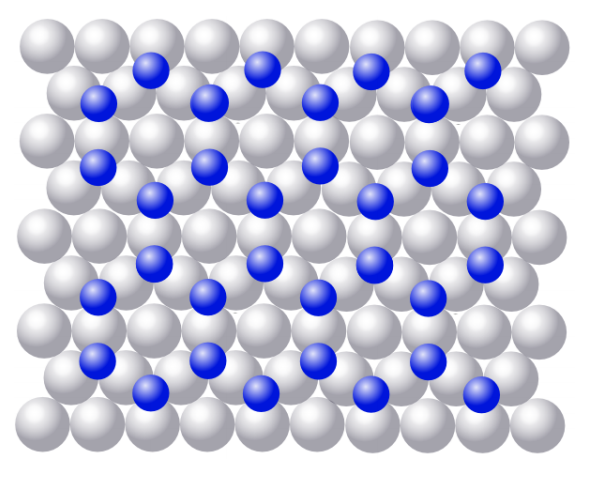
\includegraphics[width =0.9 \linewidth]{Figures/Model/Hydrogen sites.png}
        \caption{Arrangement of Hydrogen Sites
        }\label{sub@fig:hydrogen honeycomb structure}
    \end{subfigure}
    \hfill
    \begin{subfigure}{0.45\linewidth}
        \centering
        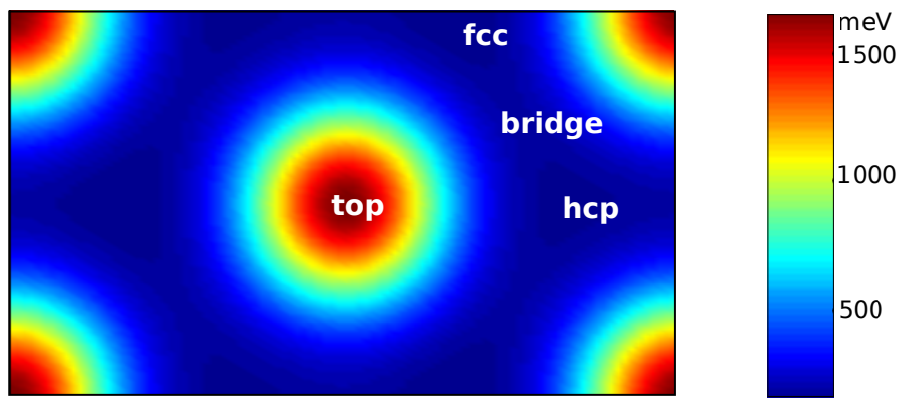
\includegraphics[width = 0.9\linewidth]{Figures/Model/Hydrogen DFT Potential.png}
        \caption{DFT Potential surface
        }\label{sub@fig:Nickel DFT surface}
    \end{subfigure}
    \caption{
        Diagrams demonstrating
        the arrangement of hydrogen
        sites on a Ni(111) surface.
        Hydrogen sites alternate
        between low energy FCC and
        high energy HCP sites arranged
        in a honeycomb structure.
        \cref{sub@fig:hydrogen honeycomb structure,sub@fig:Nickel DFT surface}
        are reproductions of those found in\cite{Jianding-Zhu}
    }
\end{figure}
To calculate the incoherent
rate of tunneling between
the FCC and HCP groundstate
we need to find a
hamiltonian describing the combined
electron-hydrogen system.
This can be split into free and interaction energy
\begin{equation}
    \hat{H} = \hat{H}_{free} + \hat{H}_{int}
\end{equation}
where the free hamiltonian \(\hat{H}_{free}\)
can be separated
into an electron and hydrogen component
\begin{equation}
    \hat{H}_{free} =
    \hat{H}_{e^-} + \hat{H}_{h}\\
\end{equation}

\subsection{Electron States}\label{sec:electron states}
For the purpose of this model we ignore the
interaction between the electrons
and the lattice as well as electron-electron
interactions. This allows
us expand the free electron
hamiltonian using the plane wave
basis
\begin{equation}
    \hat{H}_{e^-} = \sum_{k, s}
    \frac{\hbar^2 k^2}{2m_e} \hat{b}^\dagger_{k, s} \hat{b}_{k, s}\\
\end{equation}
where \(\hat{b}^\dagger_{k, s}\)
is the electron creation operator
with spin \(s\) and wavevector
\(k\) satisfying the standard
fermion anti-commutation relations
\( \{ \hat{b}_{k, s}, \hat{b}^\dagger_{k', s'} \}
= \delta_{k k'} \delta_{s s'}\).

Taking the lattice constant of Nickel as
\(3.499\pm{}0.005\times{}10^{-10}m\)~\cite{PhysRev.25.753},
we find the density of Nickel as
\(9.34\times{}10^{28}m^{-3}\).
Assuming both of the 2 valence
electrons on Nickel are completely
delocalised in
the free electron gas we
find an electron density of
\(n = 1.87\times{}10^{29} m^{-3}\).
We then used this value to calculate
the fermi-wavevector and fermi-energy of
Nickel~\cite{KittelCharles1953Itss}
\begin{align}
    \epsilon_f & = \frac{\hbar^2}{2m} {(3\pi^2n)}^{2/3} \\
    k_f^3      & = 3 \pi^2 n
\end{align}
which gives a value of
\begin{align}
    \epsilon_f & = 1.91\times{}10^{-18}J                                  \\
    k_f        & = 1.77\times{}10^{10}m^{-1} \label{eqn:fermi wavevector}
\end{align}
From measurements of the optical
properties of Nickel the
fermi energy is found to
be slightly lower
at only
\(1.24\times{} 10^{-18}J\)~\cite{PhysRev.131.2469}.

\subsection{Hydrogen States}
For hydrogen
we make use of the
eigenstates found from
the previous DFT
analysis\cite{Jianding-Zhu}.
\begin{equation}
    \hat{H}_{h} =
    E_0 \sum_{i \exists fcc} \hat{a}^\dagger_i \hat{a}_i
    + E_1 \sum_{i \exists hcp} \hat{a}^\dagger_i \hat{a}_i
\end{equation}
where \(E_0\) is the energy of an FCC site and
\(E_1\) is the energy of a HCP site.
\(\hat{a}^\dagger_i\) is
the hydrogen creation
operator for the site i
which satisfies the standard commutation
relations for a boson
\(\left[ \hat{a}_i, \hat{a}^\dagger_j \right]
= \delta_{ij}\).

Although the DFT calculation
also provides a theoretical calculation
of the hydrogen energies, the
energy used in the
model were
taken from direct spin-echo measurements~\cite{Jianding-Zhu}.
These measurements gave a value of
\begin{equation}
    \Delta{}E_{hyd} = E_1 - E_0
    = 3.04\pm0.16\times{}10^{-21} J
    \label{eqn:hydrogen energy difference}
\end{equation}


\subsection{Electron Hydrogen Interaction}
The electron hydrogen interaction can
be described simply by introducing
the electron and hydrogen field
operators \(\hat{\psi}_e\) and
\(\hat{\psi}_h\)~\cite{nazarov_danon_2013}
\begin{equation}
    \hat{H}_{int} = \int\int{d\vec{r} d\vec{r}'
        V(\vec{r}-\vec{r}')
        \hat{\psi}^\dagger_h(\vec{r})
        \hat{\psi}^\dagger_e(\vec{r'})
        \hat{\psi}_e(\vec{r'})
        \hat{\psi}_h(\vec{r})}
\end{equation}
where \(V(\vec{r})\) is
the electron-hydrogen
interaction potential.
We first expand out the
electron operator in
the free electron basis state
\begin{align}
    \hat{\psi}_e(\vec{r}) & = \sum_{k, s}
    \braket{\vec{r}|\vec{k}}
    \hat{b}_{k, s}                                      \\
                          & = \frac{1}{L^{\frac{3}{2}}}
    \sum_{k, s} \exp{(i\vec{k}.\vec{r})}
    \hat{b}_{k, s}
\end{align}
to give us the expression
\begin{align}
    \hat{H}_{int} & =
    \sum_{k, s, k', s'} \int\int{\frac{d\vec{r} d\vec{r}'}{L^3}
        V(\vec{r}-\vec{r}')
        \hat{b}^\dagger_{k',s'}
        \hat{b}_{k, s}
        \exp{(i(\vec{k} - \vec{k'}).\vec{r'})}
        \hat{\psi}^\dagger_h(\vec{r})
    \hat{\psi}_h(\vec{r})}                       \\
                  & = \begin{aligned}[t]
        \frac{1}{L^3}
        \sum_{k, s, k', s'}
         & \int d(\vec{r}' - \vec{r})
        V(\vec{r}-\vec{r}')
        \hat{b}^\dagger_{k',s'}
        \hat{b}_{k, s}
        \exp{(i(\vec{k} - \vec{k'}).(\vec{r'} - \vec{r}))} \\
         & \int d\vec{r}
        \exp{(i(\vec{k} - \vec{k'}).\vec{r})}
        \hat{\psi}^\dagger_h(\vec{r})
        \hat{\psi}_h(\vec{r})
    \end{aligned} \\
    \hat{H}_{int} & = \frac{1}{L^3}
    \sum_{k,s,k',s'}
    \hat{b}^\dagger_{k',s'}\hat{b}_{k,s}
    \tilde{V}(\vec{q})\int{d\vec{r}
    \hat{\psi}_h^{\dagger}\hat{\psi}_h
    \exp(i\vec{q}.\vec{r})}
\end{align}
If we expand out the
hydrogen creation operator
\begin{equation}
    \hat{\psi}_h(\vec{r}) =
    \sum_{i} \psi_{h,i}(\vec{r})
    \hat{a}_i
\end{equation}
we find
\begin{equation}
    \hat{H}_{int} = \frac{1}{L^3}
    \sum_{\substack{ k,s,k',s'\\ i,j}}
    \hat{b}^\dagger_{k',s'}\hat{b}_{k,s}
    \hat{a}^\dagger_i \hat{a}_k
    \tilde{V}(\vec{q})\int{d\vec{r}
        \psi^*_{h,i}(\vec{r})\psi_{h,j}(\vec{r})
        \exp(i\vec{q}.\vec{r})}\label{eqn:interaction hamiltonian expanded}
\end{equation}
where \(\vec{q} = \vec{k} - \vec{k'}\)
is the scattering wavevector, and
\(\tilde{V}(\vec{q})\) is the
fourier transform of the interaction
potential.


\subsection{The Electron Hydrogen Potential}\label{sec:electron hydrogen potential}

The electrons surrounding the hydrogen
atom have energies
\(E_n = -\frac{13.6}{n^2} eV\)~\cite{griffiths_schroeter_2018}.
Since the energy required to excite the electron
to the \(n=2\) energy level is much greater
than the fermi energy of \(Ni\)
(\(7.76eV\)~\cite{PhysRev.131.2469}) we can
make the approximation that the electron surrounding
the hydrogen lie close to the 1s groundstate.
The potential can then be found from
the greens function of the coulomb
equation~\cite{AQP_Problems}
\begin{equation}
    V(\vec{r}) = \frac{e^2}{4 \pi \epsilon_0}(
    -\frac{1}{r}
    + \int{\frac{\abs{\psi(\vec{r}')}^2}{
            \abs{\vec{r} - \vec{r'}}} d\vec{r}'})
\end{equation}
where \(a_0\) is
the bohr radius and
\begin{equation}
    \psi(\vec{r}) = {(\pi a_0^3)}^{-1/2} e^{-\frac{r}{a_0}}
\end{equation}
is the 1s hydrogen orbital~\cite{griffiths_schroeter_2018}.
We then fourier
transform this expression
(see \cref{app:interaction potential calculation})
to find
\begin{eqnarray}
    V(\vec{q}) &=& \frac{e^2}{\epsilon_0 q^2}(
    \frac{\alpha^4}{{(\alpha^2 + q^2)}^2} - 1
    )
\end{eqnarray}
with \(\alpha = \frac{2}{a_0}\). If we expand
about \(q=0\) we find
\begin{eqnarray}
    V(q) &\sim&\frac{e^2}{\epsilon_0 q^2}(1 - 2{(\frac{q}{\alpha})}^2 + 3 {(\frac{q}{\alpha})}^4 - 1)\\
    {} &=& -\frac{2e^2}{\epsilon_0 \alpha^2}(1 - \frac{3}{2}{(\frac{q}{\alpha})}^2) + \mathcal{O}(q^4)
\end{eqnarray}
taking \(q = k_f = 1.77\times{}10^{10}m^{-1}\)
(see \cref{sec:electron states})
and \(\alpha = 3.79\times{}10^{10}\) we see the second
order correction only contributes to a variation
of around \(14.5\% \).
We therefore assume that for the relevant scattering
of electrons the potential takes a constant
value \(V(q) \sim -\frac{2e^2}{\epsilon_0 \alpha^2}\).

\subsection{The Hydrogen Wavefunction}
The final term in
\cref{eqn:interaction hamiltonian expanded}
involves the integral
of the product of the two
hydrogen wavefunctions.
The form of these wavefunctions
are known from
previous DFT Calculations\cite{Jianding-Zhu}
however the wavefunctions provided
by these calculations
are expressed in terms of bloch wavefunctions spread
through the whole material.
To recover a localised
wavepacket several of these states were chosen
centered about \(q=0\).
Given the localised wavefunction
it was then possible to calculate the fourier
transform products directly. As there was a fixed
distance between the FCC and HCP lattice
sites however the fourier transform was seen to
oscillate (\cref{fig:fourier transform oscillation}),
with a frequency proportional to
\(\frac{2\pi}{a}\) where \(a\) is the lattice
constant of Ni. The value of this constant
is around
\(3.499\pm{}0.005\times{}10^{-10}m\)~\cite{PhysRev.25.753}
corresponding to oscillations at
\(q = 1.79 \pm 0.03 \times{}10^{10}m^{-1}\).
\begin{figure}[htbp]
    \centering
    \begin{subfigure}{0.45\linewidth}
        \centering
        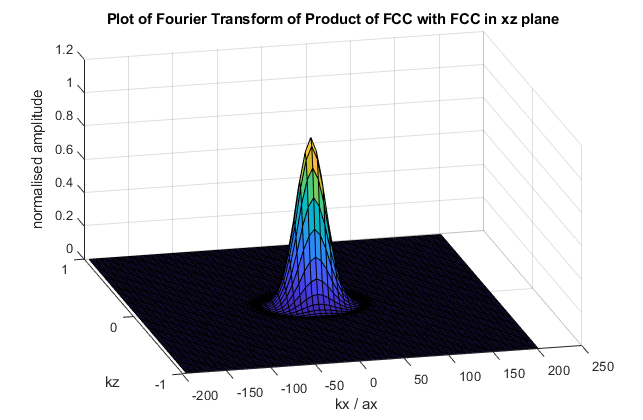
\includegraphics[width= 0.9\linewidth]{Figures/Model/Plot of fourier transform of the wavefunction fccfcc xz plane.png}
        \subcaption{FCC-FCC Fourier Transform in xz Plane}\label{fig:diagonal hydrogen matrix element no oscillation}
    \end{subfigure}
    \hfill
    \begin{subfigure}{0.45\linewidth}
        \centering
        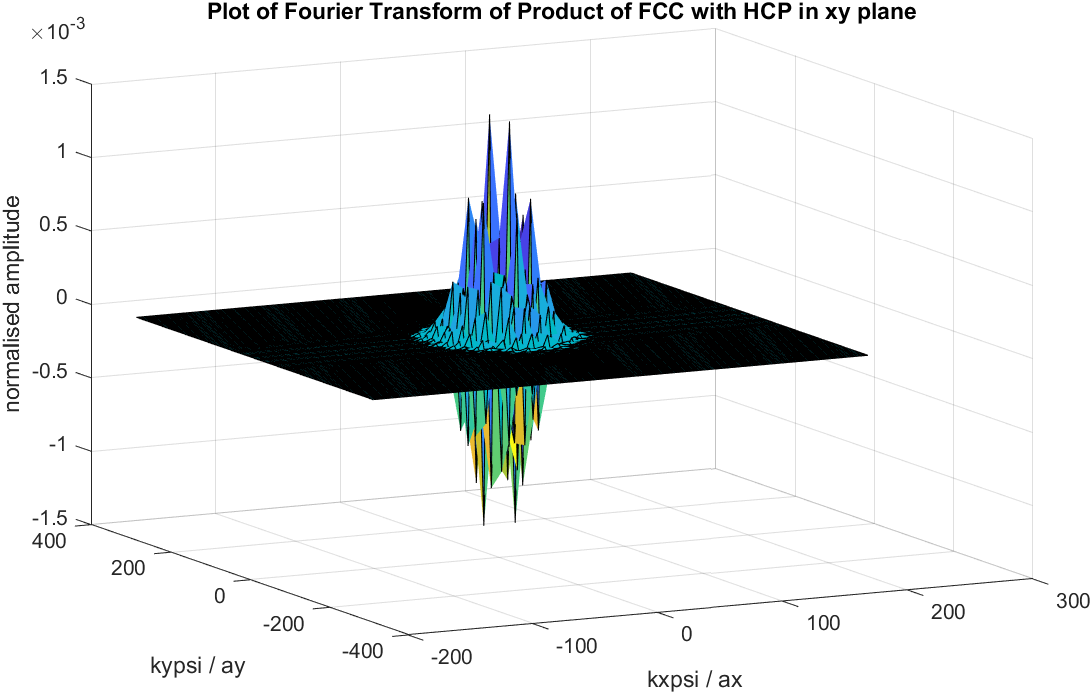
\includegraphics[width= 0.9\linewidth]{Figures/Model/Plot of fourier transform of the wavefunction.png}
        \subcaption{FCC-HCP Fourier Transform in xy Plane}\label{fig:cross hydrogen matrix element oscillation}
    \end{subfigure}
    \caption{Results of the hydrogen fourier transform calculations.
    FCC-FCC and HCP-HCP calculations
    (\cref{fig:diagonal hydrogen matrix element no oscillation})
    show a smooth curve, with a normalised
    value of one at \(q=0\).
    The FCC-HCP fourier transform
    (\cref{fig:cross hydrogen matrix element oscillation})
    however show oscillations with a characteristic
    wavevector \(q = 1.79 \pm 0.03 \times{}10^{10}m^{-1}\),
    corresponding to the lattice vector of \(Ni\).}\label{fig:fourier transform oscillation}
\end{figure}
In theory this should have a noticeable
effect on the matrix element, with a
fermi wavevector of
\(1.177\times{}10^{10} m^{-1}\)~\cref{eqn:fermi wavevector},
however since the overall wavepacket decays over a region
of around \(\frac{100\pi}{a}\) we should be
able to average over the rapid oscillations of
\(V(\vec{q})\) to obtain an effective constant
potential required for the simulation. For this
model we therefore simply take the maximum overlap
of the normalised wavefunction (\cref{tab:hydrogen overlaps}).
\begin{table}[htbp]
    \begin{center}
        \begin{tabular}{ *{3}{c} }
            \toprule
            Overlap & Maximum Overlap        & Normalised Overlap     \\
            \midrule
            FCC-FCC & \(3.00\times{}10^{7}\) & \(1\)                  \\
            HCP-HCP & \(3.00\times{}10^{7}\) & \(1\)                  \\
            HCP-FCC & \(1.33\times{}10^{5}\) & \(4.4\times{}10^{-3}\) \\
            \bottomrule
        \end{tabular}
    \end{center}
    \caption{Normalised Hydrogen overlaps as used in the
        model. Fluctuations in the overlap
        integral are ignored. The maximum
        is taken instead of the \(q=0\) value as the HCP-FCC integral
        has a minimum at this point.}\label{tab:hydrogen overlaps}
\end{table}

\subsection{Simplified Electron-Hydrogen Interaction
}\label{sec:simplified interaction}
For simplicity, in the following sections
we gather the constant terms into
an effective potential.
\begin{equation}
    \hat{H}_{int} = \sum_{k,s,k',s',i,j}
    {\tilde{V}(\vec{q})}_{i,j}
    \hat{b}^\dagger_{k',s'}\hat{b}_{k,s}
    \hat{a}^\dagger_{i}\hat{a}_{j}
    \label{eqn:interaction hamiltonian in k}
\end{equation}
If we take the potential to be independent
of \(q\) we can separate it
into a constant prefactor
and hydrogen overlap factors
\begin{align}
    V_{i,j}
     & =
    \frac{1}{L^3}
    \mathcal{C}_{i,j}
    \frac{2e^2}{\epsilon_0 \alpha^2} \\
     & =
    \frac{1}{L^3}
    \mathcal{C}_{i,j}
    \frac{8 \pi^2 \epsilon_0 \hbar^4}{e^2 m_e^2}
    \label{eqn:simplified interacton potential}
\end{align}
where \(\mathcal{C}\) takes
the value
\begin{align}
    \mathcal{C}_{i, i}      & = 1      \\
    \mathcal{C}_{i, \neq i} & = 0.0044
\end{align}

It is often beneficial to separate
\cref{eqn:interaction hamiltonian in k}
into a system and environment contribution.
\begin{align}
    \hat{H}_{int} & =
    \sum_{i,j}
    \hat{a}^\dagger_{i}\hat{a}_{j}
    \sum_{k,s,k',s'}
    \tilde{V}_{i,j}
    \hat{b}^\dagger_{k',s'}\hat{b}_{k,s} \\
                  & = \sum_{i,j}
    \hat{S}_{i,j} \hat{E}_{i,j}\label{eqn:split interaction hamiltonian}
\end{align}
where
\begin{align}
    \hat{S}_{i,j} & = \hat{a}^\dagger_{i}\hat{a}_{j} \\
    \hat{E}_{i,j} & = \sum_{k,s,k',s'}
    \tilde{V}_{i,j}
    \hat{b}^\dagger_{k',s'}\hat{b}_{k,s}
\end{align}

\section{Lindblad Equation}\label{sec:redfield}

\subsection{General Equation of Motion}
The state of the electron hydrogen
system at a given time can be completely
characterised by its density
matrix.
Working in the interaction
picture, a general density matrix
\(\hat{\rho}(t)\) time evolves according
to the von Neumann equation~\cite{TP2_Notes}.
\begin{equation}
    \frac{d\hat{\rho}_t(t)}{dt} =
    -i [\hat{H}_{int}(t), \hat{\rho}_t(t)]
    \label{eqn:density equation of motion}
\end{equation}
which can be integrated to give
\begin{equation}
    \hat{\rho}_t(t) =
    \hat{\rho}_t(0)
    - i \int_0^t ds
        [\hat{H}_{int}(s), \hat{\rho}_t(s)]
    \label{eqn:integrated density equation of motion}
\end{equation}
We can expand this equation of motion
to second order in the interaction
by substituting \cref{eqn:integrated density equation of motion}
into \cref{eqn:density equation of motion}
twice to give
\begin{equation}
    \frac{d\hat{\rho}_t(t)}{dt} =
    -i [\hat{H}_{int}(t), \hat{\rho}_t(0)]
    - \int_0^t ds
        [\hat{H}_{int}(s),
            [\hat{H}_{int}(s), \hat{\rho}_t(t)]]
    +\mathcal{O}({\hat{H}_{int}}^3)
\end{equation}
It is possible to reduce this to
an equation of motion
describing just the system by taking
a trace over the environment~\cite{Manzano_2020}
\begin{equation}
    \hat{\rho}(t) =
    -i Tr_e[\hat{H}_{int}(t), \hat{\rho}_t(0)]
    - \int_0^t ds
    Tr_e[\hat{H}_{int}(s),
    [\hat{H}_{int}(s), \hat{\rho}_t(t)]]
    \label{eqn:density motion before redfield approximation}
\end{equation}
where \(\hat{\rho}(t) = Tr_e[\hat{\rho}_t(t)]\)
is the density operator of the system.
Using a clever re-definition of the interaction
Hamiltonian~\cite{Manzano_2020} it
is possible to show that the first
term gives no contribution to the
overall dynamics of the system.

\subsection{The Redfield Assumption}\label{sec:the redfield assumption}
To arrive at the Redfield equation
we first make the assumption that the
system and surrounding density
matrix is completely
decoupled~\cite{theory_open_quantum_systems},
allowing us to write
\begin{equation}
    \hat{\rho}_t(t) = \hat{\rho}(t) \otimes \hat{\rho}_E(t)
\end{equation}
where \(\hat{\rho}_E(t)\), the
density matrix of the environment,
is taken as a purely statistical ensemble.
Under the Markov approximation
we can extend the upper limit
of \cref{eqn:density motion before redfield approximation}
to \(\infty \), arriving at the Redfield
equation
\begin{equation}
    \dot{\hat{\rho}}(t) =
    - \int_0^{\infty} ds
    Tr_{E}[\hat{H}_{int}(t),
            [\hat{H}_{int}(s-t),
                    \hat{\rho}(t) \otimes \hat{\rho}_E(t)]]
\end{equation}
Separating out the interaction hamiltonian
into system and surroundings according
to~\cref{eqn:split interaction hamiltonian}
\begin{align}
    \hat{H}_{int} & = \sum_{i,j} \hat{S}_{i,j} \hat{E}_{i,j}
\end{align}
we can simplify the form of this equation to give~\cite{Manzano_2020}
\begin{equation}
    \dot{\hat{\rho{}}}(t) = \begin{aligned}[t]
        \sum_{i,j,k, l} &
        \exp{(-i(\omega_{i,j}-\omega_{k,l})t)}
        \Gamma_{i,j;k, l}(\omega_{k,l})
        [S_{k, l}\hat{\rho}(t),
        S^\dagger_{i,j}]  \\
        +               &
        \exp{(i(\omega_{i,j}-\omega_{k,l}))}
        \Gamma^*_{k, l; i,j}(\omega_{i,j})
        [S_{k, l},
            \hat{\rho}(t) S^\dagger_{i,j}]
    \end{aligned} \label{eqn:redfield equation gamma form}
\end{equation}
where \(\Gamma \) is given by
\begin{equation}
    \Gamma_{i,j, k,l}(\omega) =
    \int_0^\infty{}{
    ds \exp{(i\omega{}s)}
    Tr_{E}[E^\dagger_{i,j}(t)E_{k,l}(t-s)\rho_E(0)]
    }\label{eqn:gamma definition}
\end{equation}

\subsection{The Lindblad Equation}
To obtain the Lindblad equation
we need to apply the rotating
wave approximation to
\cref{eqn:redfield equation gamma form}.
Before applying this
we first expand out the commutators
(reference)
\begin{equation}
    \bra{m}[S_{k, l}\hat{\rho}(t),
        S^\dagger_{i, j}] \ket{n} =
    \sum_{\alpha, \beta} \rho_{\alpha, \beta} [
        \delta_{m, k}\delta_{l, \alpha}
        \delta_{\beta, j}\delta_{i, n}
        -\delta_{m, j}\delta_{i, k}
        \delta_{l, \alpha}\delta_{\beta, n}]
\end{equation}

to

\subsection{Calculating \(\Gamma \)}
Using \cref{eqn:gamma definition}
we can calculate the value of \(\Gamma \).
The
density matrix of a purely
statistical ensemble is given
by~\cite{sakurai_napolitano_2020}
\begin{equation}
    \rho_E(0) = \sum_{\{N(k)\}}
    P(\{N(k)\})
    \ket{N(k)} \bra{N(k)}
\end{equation}
and
\begin{equation}
    \hat{E}_{i,j} = \sum_{k,s,k',s'}
    {\tilde{V}_{eff}(\vec{q})}_{i,j}
    \hat{b}^\dagger_{k',s'}\hat{b}_{k,s}
\end{equation}
where we assume the potential
is independent of \(q\). We can
take the trace over the
environment (todo reference)
\begin{equation}
    Tr_E[\dots]  = \begin{aligned}[t]
        \sum_{\substack{\{N(k)\}                             \\
        k_1,s^1,k_2,s^2                                      \\
                k_3,s^3,k_4,s^4 }}
         & P(\{N(k)\}) V_{i,j} V_{k,l}                       \\
         & \exp{(i(E_1 - E_2) t)} \exp{(i(E_3 - E_4) (t-s))} \\
         & \bra{N(k)}
        \hat{b}_{k_1,s^1}^\dagger{} \hat{b}_{k_2,s^2}
        \hat{b}_{k_3,s^3}^\dagger{} \hat{b}_{k_4,s^4}
        \ket{N(k)}
    \end{aligned}
\end{equation}
where \( \{N(k)\} \) is the set of
all possible occupations, and
the boltzmann
probability associated with a
given state is
\(P(\{N(k)\}) = \exp{(-\beta{}(E-\mu N))}\).
The trace is only non zero in two
cases
\begin{itemize}
    \item \(k_1=k_2, s^1=s^2\),
          \(k_3=k_4, s^3=s^4\)
    \item \(k_1=k_4, s^1=s^4\),
          \(k_3=k_2, s^3=s^2\) but
          \(k_1\neq{}k_2, s^1\neq{}s^2\)
\end{itemize}
and we can therefore obtain the
simplified form of the trace (reference)
\begin{equation}
    Tr_E[\dots] = \begin{aligned}[t]
        \sum_{k_1,s^1,k_3,s^3 }
         & V_{i,j} V_{k,l} [ \\
         & N_1 N_3
                + N_1 (1 - N_3) \exp{(-i(E_3 - E_1)s)}]
    \end{aligned}
\end{equation}
Integrating over \(s\) we obtain
an additional constant on the
wavevectors, and after
converting the sum into
an integral and re-adsorbing
the power of \(L^3\) into the
definition of (reference)
\begin{align}
    \Gamma_{i,j, k,l}(\omega) & =\begin{aligned}[t]
        \sum_{s^1,s^3} \int &
        \frac{d^3\vec{k}_1}{{(2\pi)}^3}
        \frac{d^3\vec{k}_3}{{(2\pi)}^3}
        V_{i,j} V_{k,l} [
        N_1 N_3 \delta_{w, 0} \frac{m}{\sqrt{k_3^2}} \\
                            & + N_1 (1 - N_3)
                \frac{m}{\sqrt{k_1^2 - 2m\omega}}
                \delta({k_3 \pm \sqrt{k_1^2 + 2m\omega}}) ]
    \end{aligned}
\end{align}
The first term is divergent (reference)
but we find no terms in the \ldots
with \(\omega = 0\).
We evaluate the second term
by expanding about the fermi
wavevector
\begin{equation}
    \Gamma_{i,j, k,l}(\omega_{k,l}) =\begin{aligned}[t]
        \sum_{s^1,s^3} \exp{(\frac{\beta \omega_{k,l}}{2})} \frac{m k_f^2 }{{(2\pi)}^4}
        V_{i,j} V_{k,l} \sqrt{\pi} \frac{2m}{\beta \hbar^2}
    \end{aligned}
\end{equation}
substituting in the expression
for v (reference)
we arrive at the final
expression for \(\Gamma \)
\begin{equation}
    \sum_{s^1,s^3} \exp{(\frac{\beta \omega_{k,l}}{2})}
    \mathcal{C}_{i,j} \mathcal{C}_{k,l}
    \sqrt{\pi} \frac{8 k_f^2 \epsilon_0^2 \hbar^3}{\beta e^4 m^2}
\end{equation}

\subsection{}
we arrive at the final form of
the Lindblad equation
for our system
\begin{equation}
    \bra{m}\dot{\hat{\rho{}(t)}} \ket{m} = \begin{aligned}[t]
        [ & 2\Gamma_{m,\neq m;m, \neq m}(\omega_{m,\neq m})\rho_{\neq m, \neq m} \\
        - & 2\Gamma_{\neq m,m;\neq m, m}(\omega_{\neq m,m})\rho_{m, m}]
    \end{aligned}
\end{equation}
where
\begin{equation}
    \Gamma_{i,j, k,l}(\omega_{k,l})   =
    \exp{(\frac{\beta \omega_{k,l}}{2})}
    \mathcal{C}_{i,j} \mathcal{C}_{k,l}
    \sqrt{\pi} \frac{32 k_f^2 \epsilon_0^2 \hbar^3}{\beta e^4 m^2}
\end{equation}

\subsection{Analytic Solution to the Rotating Wave Approximation}
Since the form of the rotating
wave approximation is a simple
rate equation with two variables
it is possible to solve it analytically
\cref{app:combined tunnelling rates}.
From the expression above we find the
forward and backward tunnelling rate as
\begin{align}
    \gamma_0 & = 2\Gamma_{1,0;0, 1}(\omega_{1,0})       \\
             & = A \exp{(\frac{\beta \omega_{0,1}}{2})}
    \mathcal{C}_{1,0} \mathcal{C}_{0,1}                 \\
    \gamma_1 & = 2\Gamma_{0,1;1, 0}(\omega_{0,1})       \\
             & = A \exp{(\frac{\beta \omega_{1,0}}{2})} \\
\end{align}
where
\(A =
\mathcal{C}_{1,0} \mathcal{C}_{0,1}
\sqrt{\pi}
\frac{64 k_f^2 \epsilon_0^2 \hbar^3}{\beta e^4 m^2}\).
This gives a combined rate of
\begin{equation}
    \gamma_0 + \gamma_1 = 2A\cosh{(\frac{\beta (E_1 - E_0)}{2})}
    \label{eqn:theoretical rate lindblad equation}
\end{equation}
for an energy difference of
\(3.04\pm0.16\times{}10^{-21} J\)
(\cref{eqn:hydrogen energy difference})
we find a tunnelling rate of
\(6.1\times{}10^{8}s^{-1}\),
corresponding to a
tunnelling time of
\(1.6\times{}10^{-9}s\).


\begin{figure}
    \centering
    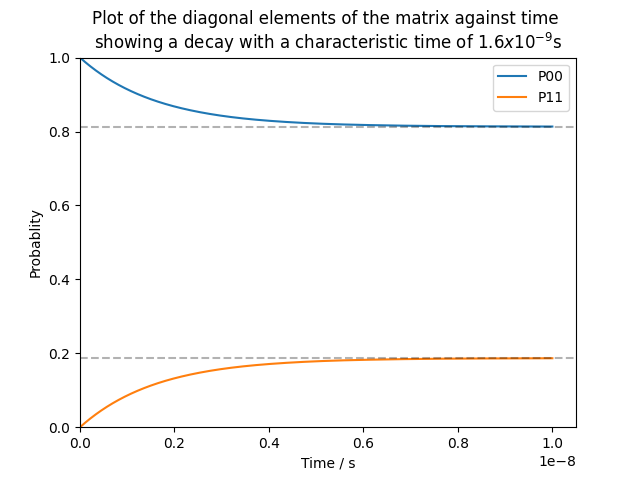
\includegraphics[width=.5\linewidth]{Figures/Redfield/Plot of lindblad solution.png}
    \caption{Plot of the Lindblad solution with a characteristic decay
    rate of \(6.1\times{}10^{8}s^{-1}\) TODO:Is this a typo???
    }\label{fig:two site lindblad soluton}
\end{figure}


\subsection{}
In reality there
are 3 HCP sites neighbouring
each FCC Hydrogen, all of which
are connected to 2 other HCP sites.
The tunnelling
rate should therefore be at least
\(3\) times the single
neighbour rate TODO CITE MODEL CHAPTER.
To investigate this behaviour we extend
the simulation to contain a large
grid of sites with periodic boundary conditions.
From this we find that the combined FCC occupation
falls at a rate of
\(1.8\times{}10^{9}s^{-1}\), exactly
three times the single neighbour rate (\cref{fig:multi site lindblad}).
\begin{figure}[htbp]
    \centering
    \begin{subfigure}{0.45\linewidth}
        \centering
        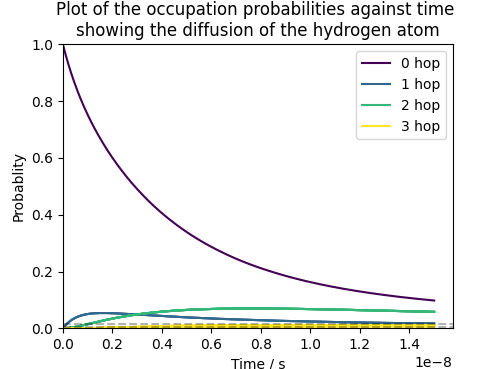
\includegraphics[width =0.9 \linewidth]{Figures/Redfield/Plot of lindblad solution many sites.png}
        \caption{Individual occupation probability
        }\label{sub@fig:multi site lindblad}
    \end{subfigure}
    \hfill
    \begin{subfigure}{0.45\linewidth}
        \centering
        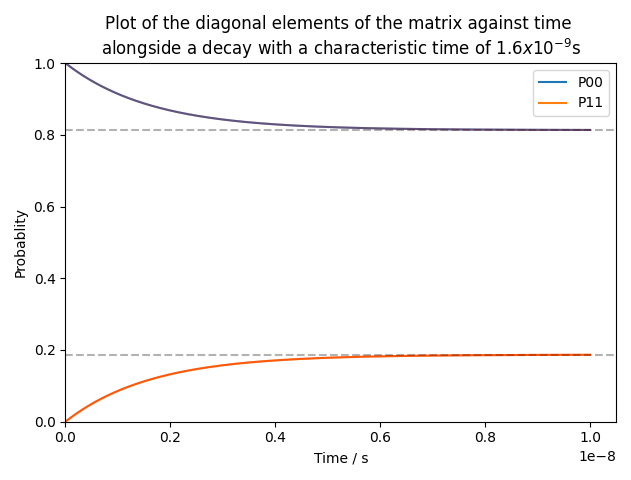
\includegraphics[width = 0.9\linewidth]{Figures/Redfield/Plot of redfield solution long time.png}
        \caption{Combined occupation probability
        }\label{sub@fig:multi site combined lindblad}
    \end{subfigure}
    \caption{Plot of the individual and combined
    occupation probabilities against time. The combined
    probability
    (\cref{sub@fig:multi site combined lindblad})
    follows exactly the same curve as in
    \cref{fig:two site lindblad soluton}
    with a rate of \(1.8\times{}10^{9}s^{-1}\).
    The plot of the individual occupation
    probabilities
    (\cref{sub@fig:multi site lindblad})
    shows that it takes
    a much longer time for the
    probability of occupation of the
    initial site to reach
    an equilibrium with the surroundings.}\label{fig:multi site lindblad}
\end{figure}
The time taken for the probability
at the initial site to reach
equilibrium is however significantly
longer, and there are several
features of the plot
which could be identified as a
tunneling time.
\begin{itemize}
    \item
\end{itemize}

And their corresponding
tunneling times are




\subsection{Extracting a Tunnelling Rate}
One issue is how best to characterise the
true tunnelling rate of this system\ldots
however the decoherent process is completely
ignored in this model

\subsection{Temperature Dependance}
\ldots we can now compare \ldots
to the temperature dependant
rates seen in experiment.

\subsection{Distance Traveled}
As well as the correct
temperature dependance
we also expect the squared
distance travelled to
grow linearly.
\begin{figure}
    \centering
    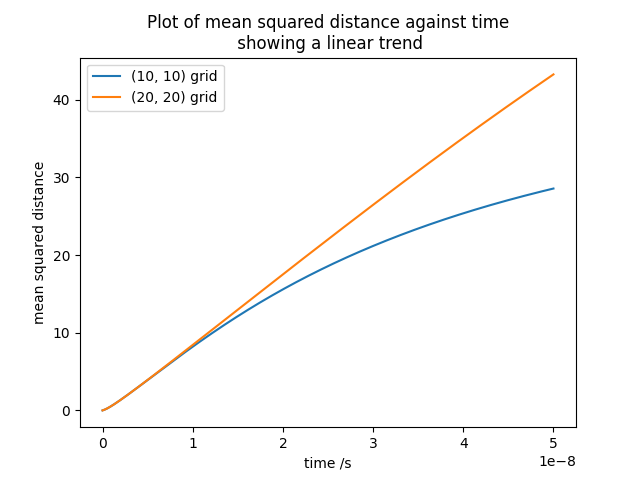
\includegraphics[width=0.5\linewidth]{Figures/Redfield/Plot of lindblad solution squared distance.png}
    \caption{Plot of the squared distance
    of the hydrogen atom against time
    showing a linear trend as expected
    for a random walk. The time taken
    for the rms distance to equal \(0.5\)
    is found to be
    \(5.25\times{}10^{-10}s\),
    which corresponds to an implied rate
    of \(1.9 \times 10^{9}s^{-1}\).
    }
\end{figure}
From this data we are able to
extract another measure
of the tunneling rate. The
time taken for the rms
distance to reach \(0.5\)
is found to be \(5.25\times{}10^{-10}s\)
giving an overall rate of
\(1.9 \times 10^{9}s^{-1}\).


\subsection{Assessing the Rotating Wave approximation}
If we relax the rotating wave approximation
we arrive at the expression given in \cref{sec:redfield equation full solution}.
\begin{align}
    \bra{m}\dot{\hat{\rho{}}}(t) \ket{n} & = \begin{aligned}[t]
        \sum_{i,j} &
        \exp{(-i\Delta{}E_{n,j;m,i} t)}
        \Gamma_{n,j;m, i}(\omega_{m,i})
        \rho_{i,j}   \\
                   &
        -\exp{(-i\Delta{}E_{i,m;i,j} t)}
        \Gamma_{i,m;i, j}(\omega_{i,j})
        \rho_{j, n}  \\
                   &
        +\exp{(i\Delta{}E_{n,j;m,i} t)}
        \Gamma_{n,j; m, i}(\omega_{n,j})
        \rho_{i, j}  \\
                   &
        -\exp{(i\Delta{}E_{i,j;i,n} t)}
        \Gamma_{i,j; i, n}(\omega_{i,j})
        \rho_{m, j}
    \end{aligned}
\end{align}
This equation produces extra oscillations
on top of the Lindblad result, with
a characteristic timescales of
\(\frac{2\pi}{\omega_{1,0}} = 2.13\times{}10^{-13}s\). Plotting
the full solution (\cref{fig:redfield full solution})
however we see exactly the same behaviour as that
predicted by the lindblad result.

\begin{figure}[htbp]
    \centering
    \begin{subfigure}{0.45\linewidth}
        \centering
        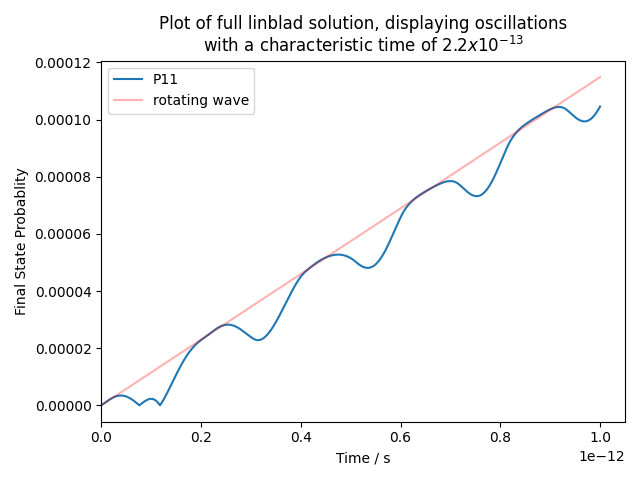
\includegraphics[width =0.9 \linewidth]{Figures/Redfield/Plot of redfield solution short time.png}
        \caption{Complete solution for small times
        }\label{fig:redfield full solution short timescales}
    \end{subfigure}
    \hfill
    \begin{subfigure}{0.45\linewidth}
        \centering
        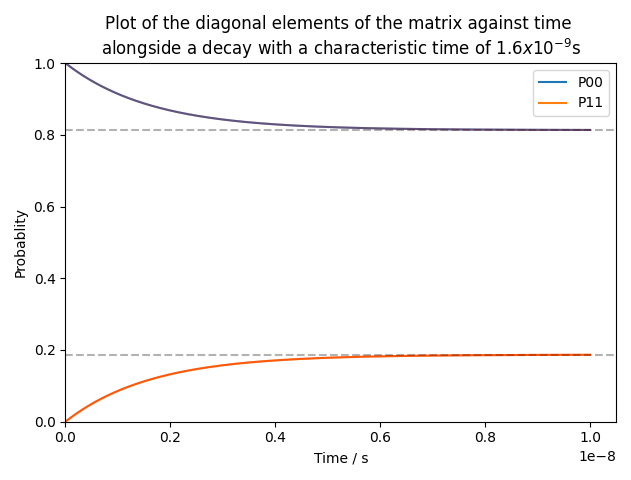
\includegraphics[width = 0.9\linewidth]{Figures/Redfield/Plot of redfield solution long time.png}
        \caption{Complete solution for long times
        }\label{fig:redfield full solution long timescales}
    \end{subfigure}
    \caption{Plot of the full solution of the Redfield
    equation. On short timescales
    (\cref{fig:redfield full solution short timescales})
    the solution is seen to
    oscillate with a characteristic
    frequency of \(2.1\times{}10^{-13}\)s however
    at long timescales (\cref{fig:redfield full solution long timescales})
    the solution decays at the same rate as the
    Lindblad equation.}\label{fig:redfield full solution}
\end{figure}

In theory we should also be able
to solve the redfield equation
for multiple hydrogen sites, however
the additional computational complexity
rules this out. It is however possible to
approximate the behaviour
seen in the many site model
by placing a sink at
the HCP site
(\cref{fig:redfield full solution with sink}).
In this case
we again see good
agreement with the
lindblad equation.
\begin{figure}[htbp]
    \centering
    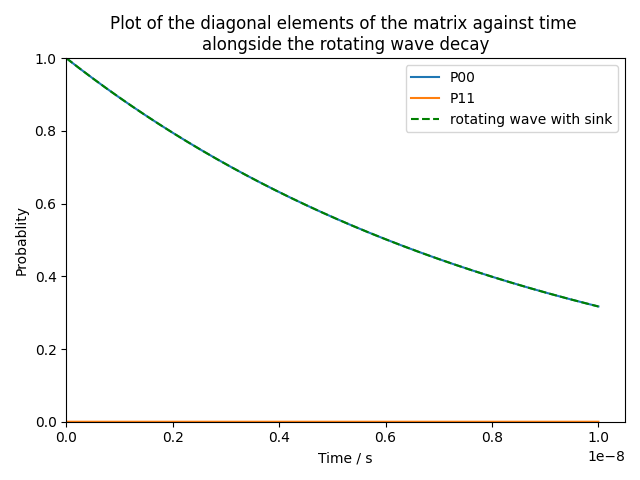
\includegraphics[width =0.45 \linewidth]{Figures/Redfield/Plot of redfield solution long time sink.png}
    \caption{Plot of the full solution of the Redfield
        equation with a sink on the HCP site.
        The hydrogen behaves exactly the same
        as in the previous lindblad analysis.}
\end{figure}



\subsection{Further Generalisations}
One issue with this approach is that it
completely ignores correlations
between the system and the surroundings.
This contradicts
one of the key features seen in the simulation;
the tunnelling process is dominated by
transitions between two states with the same energy,
rather than two states with the same electron configuration.
It is not possible to `trace out' the environment
for an arbitrary coupling, however if
we limit ourselves to
\begin{equation}
    \hat{\rho}_t = \sum_{m,n} \hat{\rho}_{m,n} \otimes {(\hat{\rho}_E)}_{m,n} \
\end{equation}
we can follow the same procedure as in
\cref{sec:the redfield assumption}
to arrive at the modified redfield equation
\begin{equation}
    \bra{m}\dot{\hat{\rho}}(t)\ket{n} = \begin{aligned}[t]
        \sum_{i,j,k, l} &
        \exp{(-i(\omega_{i,j}-\omega_{k,l})t)}
        \Gamma^{m,n}_{i,j;k, l}(\omega_{k,l})
        [S_{k, l}{\hat{\rho}(t)}_{m,n},
        S^\dagger_{i,j}]  \\
        +               &
        \exp{(i(\omega_{i,j}-\omega_{k,l}))}
        {\Gamma^*}^{m,n}_{k, l; i,j}(\omega_{i,j})
        [S_{k, l},
                {\hat{\rho}(t)}_{m,n} S^\dagger_{i,j}]
    \end{aligned}
\end{equation}
where
\begin{equation}
    \Gamma^{m,n}_{i,j, k,l}(\omega) =
    \int_0^\infty{}{
    ds \exp{(i\omega{}s)}
    Tr_{E}[E^\dagger_{i,j}(t)E_{k,l}(t-s)
    {(\hat{\rho}_E)}_{m,n}]
    }
\end{equation}
The problem is then how best to express
both the statistical and quantum uncertainty
in the form of a density matrix.

\subsection{Energy Conservation}
TODO- Reduced Temperature density matrix

TODO- How do we produced thematised and localised states??
we can do one but not both??
TODO- we want states to lie close to the fermi level after
perturbation




\section{Simulation Investigation}\label{sec:simulation}
The dynamics of the electrons
discussed in \cref{sec:the model}
can be investigated by
directly simulating the system.

\subsection{Eigenvalue Decomposition}
To simulate the system we must solve
the Schrödinger equation. This
can be done through direct
integration, however
if we first decompose
the initial state
into eigenstates
of the complete hamiltonian\cite{conduit}
\begin{align}
    \ket{\Psi(t)} = \exp{(-i\frac{Ht}{\hbar})} \sum_n C_n \ket{n} \\
    = \sum_n C_n \exp{(-i\frac{E_n t}{\hbar})} \ket{n}
\end{align}
we can propagate
by multiplying each eigenstate
by a phase-factor.

Since we are dealing with a
large number of eigenstates
it is important to think
about both the storage
and computational complexity
of the two methods (\cref{tab:algorithm complexity}).
\begin{table}[htbp]
    \begin{center}
        \begin{tabular}{ *{3}{c} }
            \toprule
            Cost    & Integration            & Decomposition              \\
            \midrule
            Time    & \(\mathcal{O}(n^2 t)\) & \(\mathcal{O}(n^3 + n d)\) \\
            Storage & \(\mathcal{O}(n d)\)   & \(\mathcal{O}(n^2 + n d)\) \\
            \bottomrule
        \end{tabular}
    \end{center}
    \caption{Complexity associated with the
        two methods of solving Schrödinger equation,
        where \(n\) is the number of eigenstates, t
        is the number of timesteps and d is the
        number of datapoints. The method
        of eigenvalue decomposition
        prevents the \(\mathcal{O}(t)\)
        dependence seen
        in direct integration
        by first decomposing the
        eigenstate (\(\mathcal{O}(n^3)\))
        before multiplying
        by the relevant phase
        (\(\mathcal{O}(nd)\)).
    }\label{tab:algorithm complexity}
\end{table}

As we
are only interested in the
evolution of the eigenstates
at times much greater than
the frequency of the sates
\(\omega = \frac{E}{\hbar}\)
the method of integration
was found to be much
slower than that of eigenvalue
decomposition. One
issue with this method
is the increased storage
cost associated with
storing the complete
hamiltonian. This could
be prevented by
working with a sparse
matrix, however in
practise this
was not required.

Although the decomposition is
expensive it was only repeated once,
which allowed us to gather a large
number of times at very little additional
cost. It was also possible to use the
fact that the matrix was hermitian to
provide and additional increase in speed.

\subsection{Matrix Representation}\label{sec:state representation}
Working in the unperturbed electron basis
(\cref{sec:electron states})
we label each eigenstate
according to the index of the
hydrogen site and
the configuration of the
electron system.
In general for \(n\)
electron states
and \(m\) hydrogen states
there would
be \(m 2^n\)
possible configurations,
however since the hamiltonian
conserves particle number
we limit ourselves
to a fixed
number of electrons (\(N\)).
In this case the number
of states scales as \(m \times{} \binom{n}{N}\).
In practise we are able to
simulate a system with
around \(3500\) eigenstates,
or \(14\) half filled electron states
(\cref{tab:number of eigenstates}).
This was limited more by
storage than CPU time, and as such it may
be necessary to investigate
the use of sparse matrices if a
larger system is required.
\begin{table}[htbp]
    \begin{center}
        \begin{tabular}{ *{4}{c} }
            \toprule
            Number of States & All Configurations & Half Filled & 2 electrons \\
            \midrule
            \(10\)           & \(1024\)           & \(252\)     & \(45\)      \\
            \(12\)           & \(4096\)           & \(924\)     & \(66\)      \\
            \(14\)           & \(16384\)          & \(3432\)    & \(91\)      \\
            \(16\)           & \(65536\)          & \(12870\)   & \(120\)     \\
            \bottomrule
        \end{tabular}
    \end{center}
    \caption{
        Number of eigenstates required
        to store an electron system.
        Limiting ourselves to
        configurations with a fixed
        number of electrons we are
        able to simulate a larger
        number of states.
        This method scales particularly
        well for a system with a
        low number of electrons
        or a low number of holes.
    }\label{tab:number of eigenstates}
\end{table}

The process of converting
between these labels and
the states used in the hamiltonian
was handled by
an ElectronSystem object (TODO reference)


When working with
fermions we need to take
care over the exchange
statistics of the hamiltonian.
For self consistency we work in
a basis such that electrons
with lower energy are always
added first. Terms in the interaction
hamiltonian therefore pick
up a minus sign when there is
an odd number of electrons
between the exchanged energy levels.
\begin{align}
    a^\dagger_1a_2 \ket{2,3} & = \ket{1,3}  \\
    a^\dagger_1a_3 \ket{2,3} & = -\ket{1,2}
\end{align}
To find the probability
of finding the hydrogen in site \ldots

\subsection{Choosing the Initial States}

\subsubsection{Distribution Of Energies}
The distribution of electron energies was
initially chosen using an even spacing,
however this lead noise caused
by rabi oscillations
at a frequency
fixed through several runs
of the simulation.
To remove these oscillations
random offsets were introduced
into the energy distribution
which changed the rabi frequency
between runs,
allowing for cancellation
of the noise.

The spacing of electron energies is also
important for the simulation, as it
sets the effective volume of the Nickel
lattice. The density of states of a free electron
gas \(g(E)\) is given by~\cite{KittelCharles1953Itss}
\begin{equation}
    g(E) = \frac{V}{2\pi^2}
    {(\frac{2m}{\hbar^2})}^{\frac{3}{2}}
    E^{\frac{1}{2}}
\end{equation}
We therefore invert this expression
to find the implied volume of the
simulation
\begin{equation}
    V = 2\pi^2
    \frac{g(E)}{E^{\frac{1}{2}}}
    {(\frac{\hbar^2}{2m})}^{\frac{3}{2}}
\end{equation}
Since at large \(k\)
(for \(k\sim k_f\))
the density of states is roughly
constant we make the approximation
\begin{equation}
    g(E) = \frac{dN}{dE} \sim \frac{1}{E_{space}}
\end{equation}
where \(E_{space}\) is the energy spacing
of the simulation. From \cref{eqn:simplified interacton potential} we find
\begin{equation}
    \hat{H}_{int} \propto \frac{1}{V} \propto E_{space}
    \label{eqn:energy spacing dependance of interaction hamiltonian}
\end{equation}
for smaller
energy spacing we have
a larger volume, and a smaller
perturbation.

\subsubsection{Distribution Of Electrons}
To be able to average over successive
simulations we also need to setup the
simulation with a somewhat random
choice of initial states.
We can start the hydrogen
in the FCC site by setting the
amplitudes of the HCP sites to zero
before choosing the FCC aptitudes according to
a normal distribution.

In simulations for which we choose states
with a large range of energies however
the electron distribution should not be
random and should follow the fermi dirac distribution.
To match this distribution we
need to alter the averages used
to produce the initial state vector.
Since the amplitude corresponds to
the square-root of the probability we
take the average magnitude as the
square-root of the boltzmann probability
associated with each state.
\begin{align}
    P_k & = \exp(-\beta{}E_k)     \\
    C_k & = \exp(-\beta{}E_k / 2)
\end{align}
where \(C_k\) is the wavefunction amplitude.
If we plot the resulting
electron distribution produced
by this method for fixed N
we see the expected electron
distribution for a standard electron
gas (\cref{fig:correct fermi dirac}).
\begin{figure}[htbp]
    \centering
    \begin{subfigure}{0.45\linewidth}
        \centering
        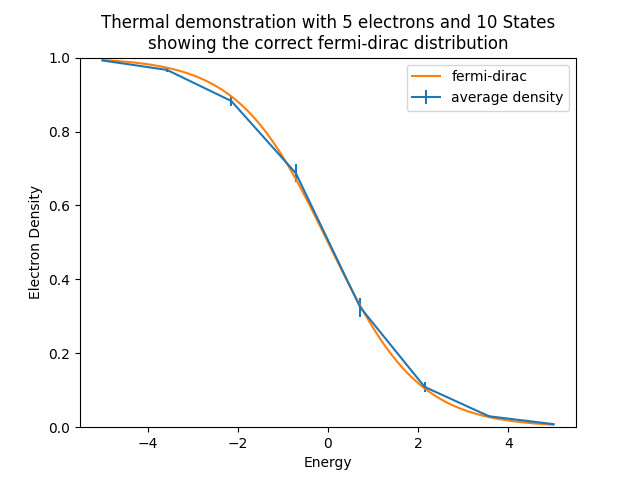
\includegraphics[width =0.9 \linewidth]{Figures/Simulation/Plot of correct fermi dirac distribution on center.png}
        \caption{5 Electrons 10 States}
    \end{subfigure}
    \hfill
    \begin{subfigure}{0.45\linewidth}
        \centering
        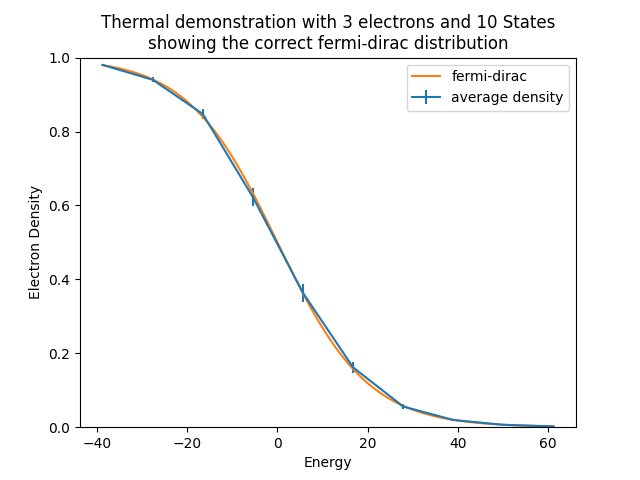
\includegraphics[width = 0.9\linewidth]{Figures/Simulation/Plot of correct fermi dirac distribution off centre.png}
        \caption{3 Electrons 10 States}
    \end{subfigure}
    \caption{Plot of the electron distribution seen
        when setting up the system randomly. The
        correct fermi-dirac distribution is seen in both the on and
        off center systems. Errors are given by the standard
        deviation of the electron densities, and are therefore
        larger around the fermi surface where fluctuations are
        large.}\label{fig:correct fermi dirac}
\end{figure}
However if we were to include
a large interaction term, such
as those required for the
real Nickel system the
electron distribution is
seen to diverge, as the approach
does not account for the
shift in the perturbed
energies (\cref{fig:incorrect fermi dirac}).
\begin{figure}[htbp]
    \centering
    \begin{subfigure}{0.45\linewidth}
        \centering
        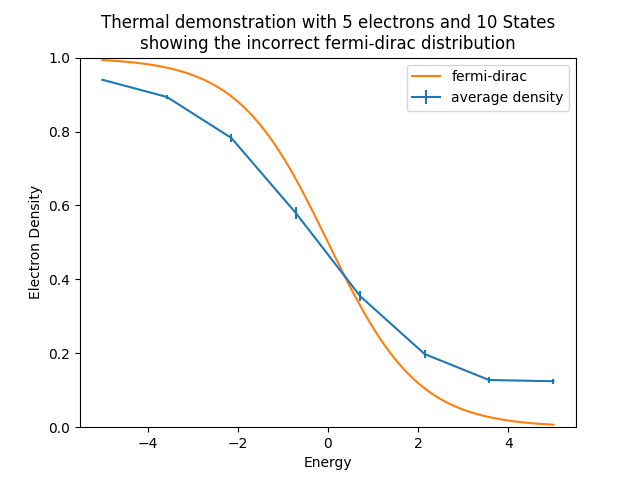
\includegraphics[width =0.9 \linewidth]{Figures/Simulation/Plot of incorrect fermi dirac distribution on center.png}
        \caption{Large interaction}
    \end{subfigure}
    \hfill
    \begin{subfigure}{0.45\linewidth}
        \centering
        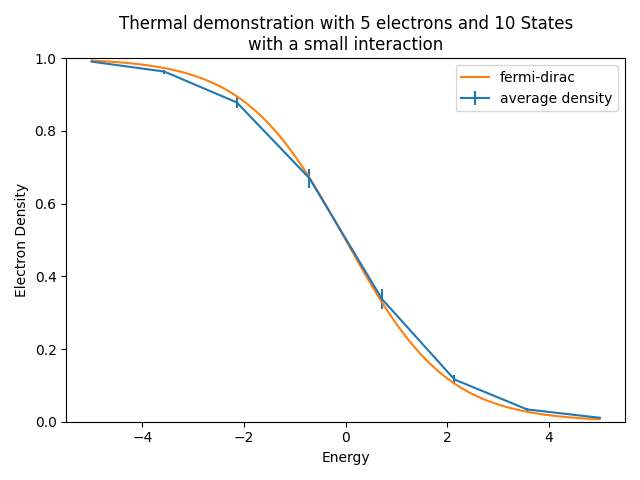
\includegraphics[width = 0.9\linewidth]{Figures/Simulation/Plot of incorrect fermi dirac distribution on center small interaction.png}
        \caption{Reduced Interaction}\label{sub@fig:reduced interaction fermi-dirac}
    \end{subfigure}
    \caption{Plot of the fermi-dirac distribution
        with the inclusion of interaction. The
        correct distribution is no longer seen when
        the full interaction is included, however
        if this is reduced by a factor of \(10\)
        (\cref{sub@fig:reduced interaction fermi-dirac})
        the correct distribution is recovered.}\label{fig:incorrect fermi dirac}
\end{figure}
To overcome this limitation
the simulation was repeated
for small energy bands (\cref{sec:small band approach})
for which the electron distribution
was uniform.

Full code is available in the appendix TODO-

\subsection{Initial Investigation}
To obtain a rough estimate of
the rate the system was setup
with electrons evenly spaced
in the region \(E_k = E_f \pm 2K_b T\)
with degenerate hydrogen energies (\cref{fig:tunnelling rate single large band}).
The hydrogen occupation
could then be inferred by
summing the occupation
of electrons in both the FCC and
HCP sites.
\begin{figure}[htbp]
    \centering
    \begin{subfigure}{0.45\linewidth}
        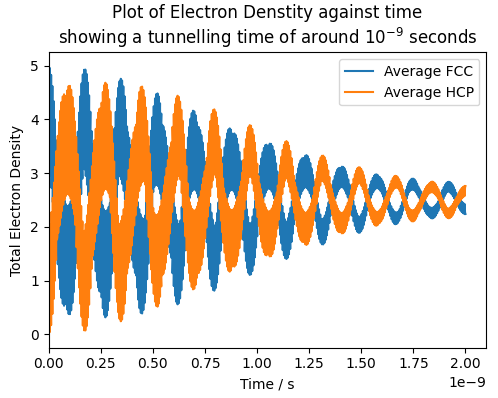
\includegraphics[width=0.9\linewidth]{Figures/Simulation/Plot of large band simulation decay times.png}
        \subcaption{Tunnelling excluding hydrogen energy}\label{fig:large band degenerate simulation}
    \end{subfigure}
    \hfill
    \begin{subfigure}{0.45\linewidth}
        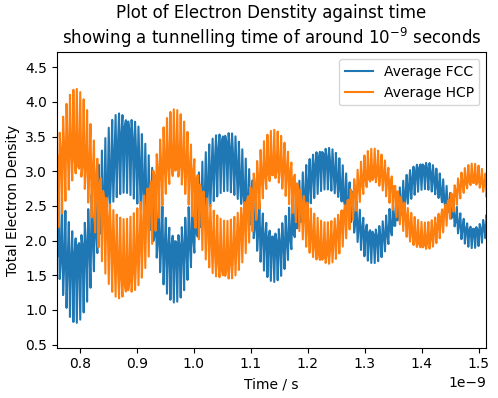
\includegraphics[width=0.9\linewidth]{Figures/Simulation/Plot of large band simulation decay times rapid oscillations.png }
        \subcaption{Rapid oscillation of the hydrogen occupation}
    \end{subfigure}
    \caption{Plot of the tunnelling rate taken using a
        simple choice of electron energies,
        taken evenly in the range \(E=E_f \pm 2 K_b T\).
        Simulation with a degenerate hydrogen
        (\cref{fig:large band degenerate simulation})
        shows tunnelling in around
        \(10^{-9}s\). TODO-Change title of plot}\label{fig:tunnelling rate single large band}
\end{figure}
Unfortunately we find that the interaction is
relatively large. The diagonal terms in
the interaction hamiltonian
had a value of \(6.21\times{}10^{-21}J\)
and a cross diagonal value of \(2.73\times{}10^{-23}J\)
whereas the electron energies were separated
by only \(9.2\times{}10^{-22}J\). This meant that
the perturbation approximation required for
fermi-dirac distributed states is not valid.
We also fail to see any tunnelling when
the hydrogen energy is included (\cref{fig:issues with single large band}).
\begin{figure}[htbp]
    \centering
    \begin{subfigure}{0.45\linewidth}
        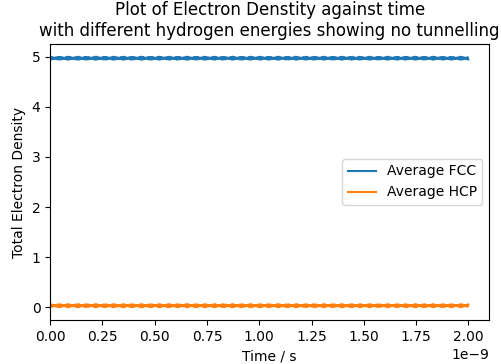
\includegraphics[width=0.9\linewidth]{Figures/Simulation/Plot of large band simulation with hydrogen energies.png}
        \subcaption{Tunnelling including hydrogen energy}\label{fig:large band non degenerate simulation}
    \end{subfigure}
    \hfill
    \begin{subfigure}{0.45\linewidth}
        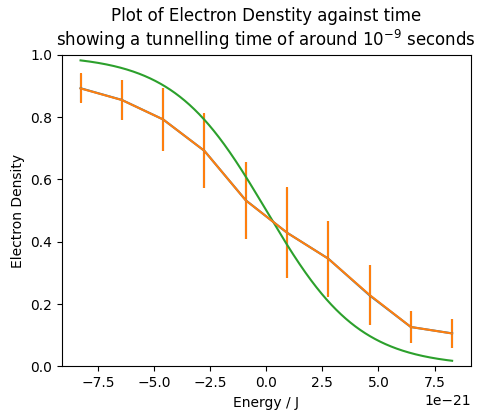
\includegraphics[width=0.9\linewidth]{Figures/Simulation/Plot of large band electron distribution.png}
        \subcaption{Electron Distribution}\label{fig:large band fermi-dirac}
    \end{subfigure}
    \caption{Plot demonstrating the issues with the
        simple approach used to calculate the rate.
        When including the hydrogen energies
        (\cref{fig:large band non degenerate simulation})
        no tunnelling can be seen, even
        at much larger timescales. Even without the
        inclusion of hydrogen energies
        the incorrect electron distribution is
        seen (\cref{fig:large band fermi-dirac}).
        TODO-Plot Title}\label{fig:issues with single large band}
\end{figure}

\subsection{Small Band Approach}\label{sec:small band approach}
To limit the effect of the incorrect
electron distribution we can
take electrons localised
in a small region of the fermi
surface such that their energies
and occupations are all similar.

One issue is that states at the edge
of the band will be `missing'
states to mix with during the
perturbation. We can approximate
this overlap using first order perturbation theory.
\begin{equation}
    \ket{n} = \ket{n^{(0)}} + \sum_{K\neq{}n} \frac{\bra{k^{(0)}} \hat{H}_{int} \ket{n^{(0)}}}{E_n^{(0)} - E_k^{(0)}} \ket{k^{(0)}}
\end{equation}
Since \(\hat{H}_{int} \propto E_{space}\)
(\cref{eqn:energy spacing dependance of interaction hamiltonian})
the degree of overlap of neighbouring states does
not depend on the energy spacing. Luckily
however the interaction is small
enough such that states only interact with
their closest neighbours (\cref{fig:single band energies}),
and the effect of these missing states should be small.
\begin{figure}[htbp]
    \centering
    \begin{subfigure}{0.45\linewidth}
        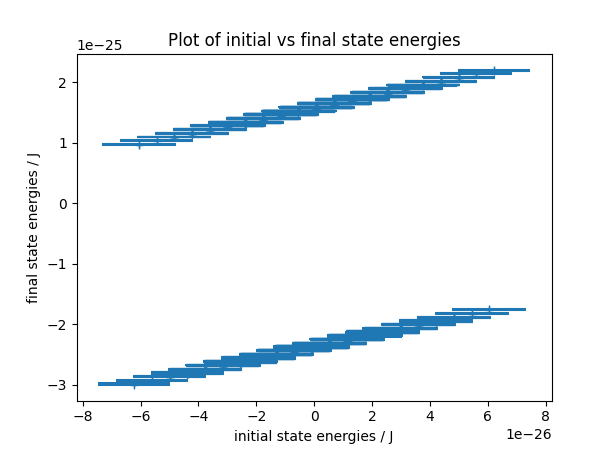
\includegraphics[width=0.9\linewidth]{Figures/Simulation/Plot of single band eigenstate energy range.png}
        \subcaption{Final State Energies}\label{fig:initial and final state energies of single band}
    \end{subfigure}
    \hfill
    \begin{subfigure}{0.45\linewidth}
        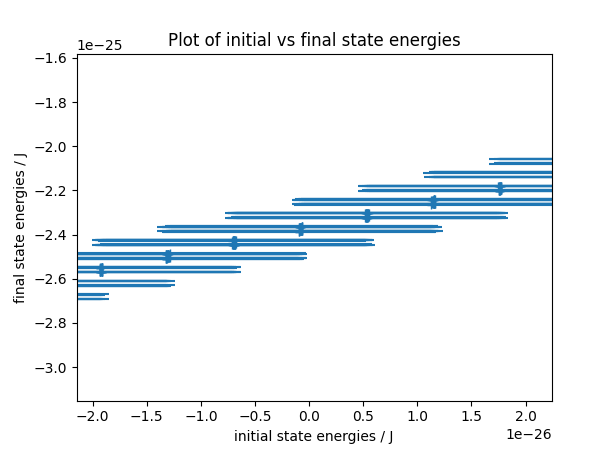
\includegraphics[width=0.9\linewidth]{Figures/Simulation/Plot of single band eigenstate energy range closeup.png}
        \subcaption{Detailed view of lower energies}\label{fig:initial and final state energies of single band zoom}
    \end{subfigure}
    \caption{Plot of average initial state energy weighted by the
        probability of occupation. The final
        state energy is separated into two,
        due to the symmetric and antisymmetric
        contributions
        (\cref{fig:initial and final state energies of single band}).
        In \cref{fig:initial and final state energies of single band zoom}
        we can see each state is highly degenerate, and mixing
        is limited to the four nearest neighbours.
    }\label{fig:single band energies}
\end{figure}


The tunneling could also be
influenced by these states
through a combination of
several electron `hops'.
Due to the energy time uncertainty
principle \(\Delta{}E\Delta{}T \geq \frac{\hbar}{2}\)
we expect the total energy to be conserved
to within
\begin{equation}
    \Delta{}E \sim \frac{\hbar}{2\Delta{} t}
\end{equation}
so that for a tunnelling time of
\(\sim 10^{-9}s\)
we expect an energy fluctuation
of \(\sim 5\times{}10^{-26} J\).
We therefore choose states separated
by at-least \(10^{-25} J\) such that
interaction with states outside
the band is prohibited
through energy conservation.


\subsection{Different Hydrogen Energy}\label{sec:different hydrogen energy}
If we add the hydrogen energies to the
simulation we no longer see tunnelling
on any timescale. Repeating the analysis
in \cref{sec:small band approach} we
see that eigenstate mixing and hence
tunnelling is dominated by
eigenstates degenerate in energy.
In the initial approach we therefore
miss many of the states which could
contribute to tunnelling. To ensure that we always have
states degenerate in energy we
therefore introduce two electron
bands separated by the hydrogen energy
difference.
\begin{figure}[htbp]
    \centering
    \begin{subfigure}{0.45\linewidth}
        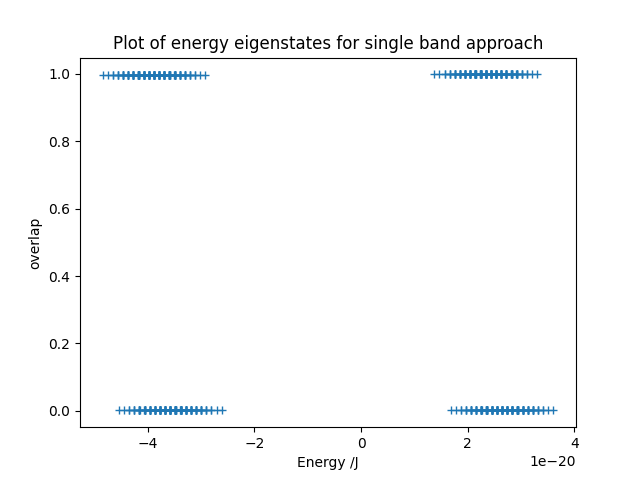
\includegraphics[width=0.9\linewidth]{Figures/Simulation/single band eigenstate energies.png}
        \subcaption{One Band Overlaps}\label{fig:one band overlap}
    \end{subfigure}
    \hfill
    \begin{subfigure}{0.45\linewidth}
        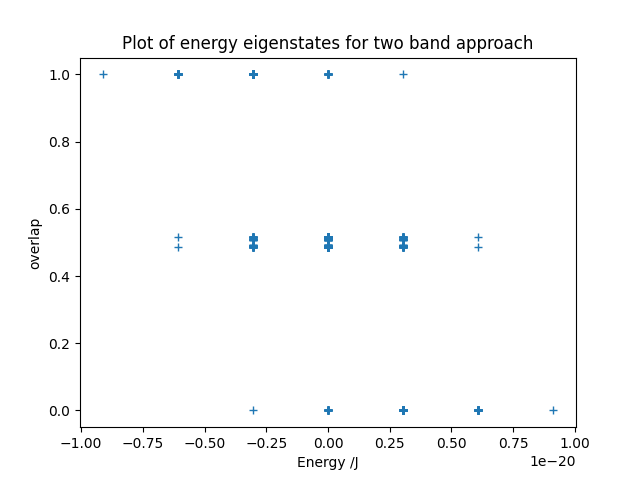
\includegraphics[width=0.9\linewidth]{Figures/Simulation/two band eigenstate energies.png}
        \subcaption{Two Band Overlaps}\label{fig:two band overlap}
    \end{subfigure}
    \caption{Plot of the energies of the
        eigenstates, against the portion of the
        state which lies in the FCC site.
        For the single band approach we
        see very little overlap between the FCC and HCP
        initial states (\cref{fig:one band overlap})
        as the energies of the FCC and HCP sites
        are poorly matched. By introducing
        two bands separated by the hydrogen energy
        difference (\cref{fig:two band overlap})
        we find mixing between states which are
        degenerate in energy
    }\label{fig:overlap with hydrogen energies}
\end{figure}

If we were to plot the initial and final
state energies for the single band approach
we no longer see two distinct levels. Instead
we see three levels split into
several distinct groups.
To promote interaction between each group
we could increase the width of each band,
however this leads to a reduction in
the overlap between states. This is
caused by different mixing
within each band which prevents
the energy degeneracy. To solve this
we could simply remove the diagonal
interaction, however in (\cref{sec:tunnelling no diagonal})
we find this effects the
measured tunneling times.
Even when
working with a small band
we do not see the desired equilibrium
behaviour, calculated assuming the rate
scales as \(N(1-N)\).
\begin{figure}[htbp]
    \centering
    \begin{subfigure}{0.45\linewidth}
        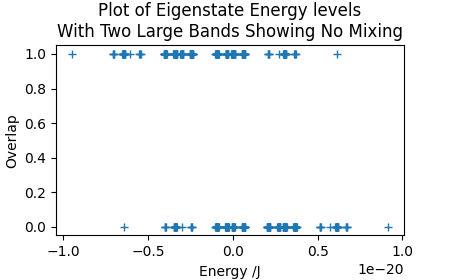
\includegraphics[width=0.9\linewidth]{Figures/Simulation/Two Large Bands No Mixing.png}
        \subcaption{Large Band Mixing}\label{fig:two band minimum mixing}
    \end{subfigure}
    \hfill
    \begin{subfigure}{0.45\linewidth}
        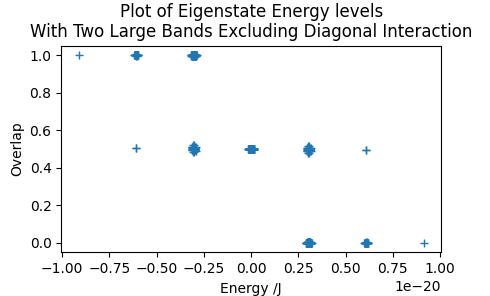
\includegraphics[width=0.9\linewidth]{Figures/Simulation/Two Large Bands No Diagonal.png}
        \subcaption{Large Band No Diagonal}\label{fig:two band no diagonal}
    \end{subfigure}
    \begin{subfigure}{0.45\linewidth}
        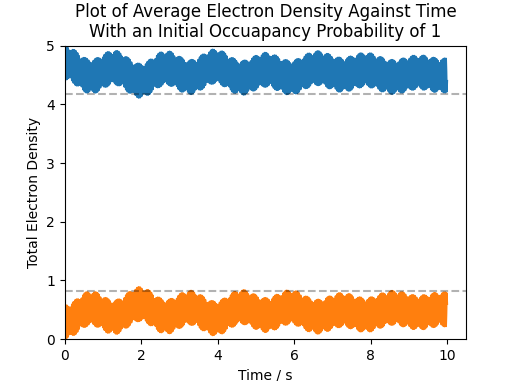
\includegraphics[width=0.9\linewidth]{Figures/Simulation/Two Small Bands Large Probability Incorrect Equilibrium.png}
        \subcaption{Large Initial Occupation}\label{fig:two band incorrect equilibrium above}
    \end{subfigure}
    \hfill
    \begin{subfigure}{0.45\linewidth}
        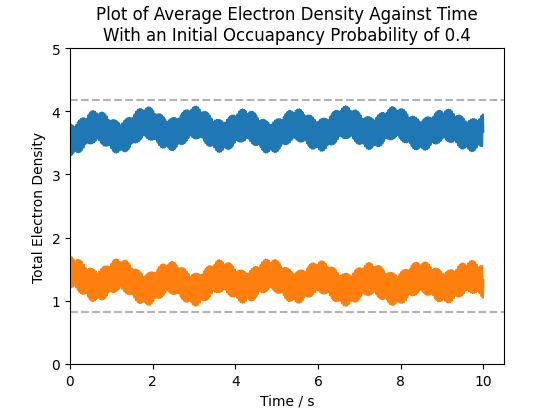
\includegraphics[width=0.9\linewidth]{Figures/Simulation/Two Small Bands Small Probability Incorrect Equilibrium.png}
        \subcaption{Small Initial Occupation}\label{fig:two band incorrect equilibrium below}
    \end{subfigure}
    \caption{
        Plots demonstrating the issues
        with the two band approach.
        \cref{fig:two band minimum mixing}
        demonstrates the issue with
        using a large band; the diagonal
        interaction causes mixing within
        groups of eigenstates which
        lifts the degeneracy required for
        the off diagonal interaction.
        This can be fixed by removing
        the diagonal interaction
        (\cref{fig:two band no diagonal})
        however in
        \cref{sec:tunnelling no diagonal}
        we find this is
        necessary for the correct
        tunneling behaviour.
        Even with a small band
        the
        predicted equilibrium
        behaviour is not seen
        (\cref{fig:two band incorrect equilibrium above,fig:two band incorrect equilibrium below}).
        There is therefore very
        little evidence that
        this method would
        approximate the true
        electron-hydrogen dynamics.
    }\label{fig:issue with two band approach}
\end{figure}
Interestingly we do see a reduction in
fluctuations if the system is initially
prepared with this occupation
(\cref{fig:two band close to equilibrium}).
We also find the material cools
as the hydrogen tunnels, as can be seen
through the average electron distribution in
the initial and final state. This is a
result of energy transfer from the
electron gas to the hydrogen
(\cref{fig:two band temperature shift}).

\begin{figure}[htbp]
    \centering
    \begin{subfigure}{0.45\linewidth}
        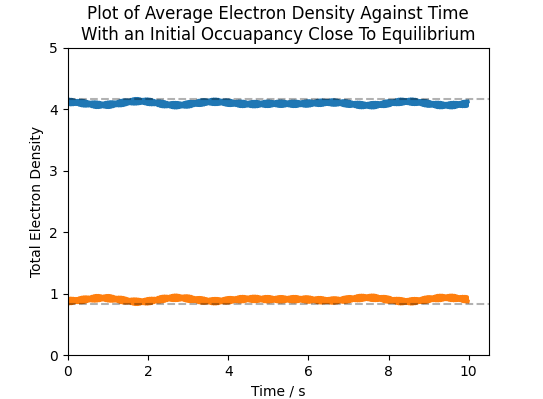
\includegraphics[width=0.9\linewidth]{Figures/Simulation/Two Small Bands Probability Clsoe To Equilibrium.png}
        \subcaption{Evoulution Close To Equilibrium}\label{fig:two band close to equilibrium}
    \end{subfigure}
    \hfill
    \begin{subfigure}{0.45\linewidth}
        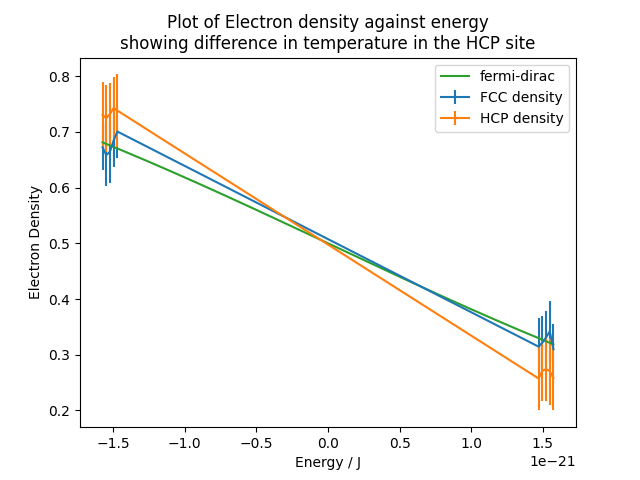
\includegraphics[width=0.9\linewidth]{Figures/Simulation/two band electron distribution.png}
        \subcaption{Two Band Electron Distribution}\label{fig:two band temperature shift}
    \end{subfigure}
    \caption{
        Interesting features of the two
        band dynamics.
        In \cref{fig:two band close to equilibrium}
        we find noise is reduced when the
        hydrogen is prepared in a state
        close to the predicted equilibrium
        occupation. This suggests it is
        true equilibrium of the
        system.
        In \cref{fig:two band temperature shift}
        the temperature shift can be seen.
        This is a consequence of energy transfer
        between the electron gas to the
        hydrogen. The temperature
        shift can be reduced by adding
        more electrons to the
        simulation.
    }\label{fig:final notes two band}
\end{figure}

\FloatBarrier\
\section{Simulation Results}\label{sec:simulation results}

From the previous investigation it is clear
that it is not possible to directly
incorporate the hydrogen energy
into the simulation.
The only key difference
between degenerate and
non-degenerate tunneling
however
is the location of the
electrons
immediately after
tunneling. Since
mixing only occurs
between states degenerate
in energy we expect
to see a lower energy
distribution in the
HCP site, however
in the
limit of a large
number of electrons
this energy
difference is negligible.
Since the off diagonal
interaction is small
we also find that the
individual electrons
transition at a much
faster rate than
hydrogen, and it is
reasonable
to expect that
the exact electron
distribution after a
transition has no effect
on the hydrogen dynamics.
This is the same reason that
we are able to assume separability
of the electron and hydrogen
density matrices in
\cref{sec:the redfield assumption}.
The electron distribution
during a transition however
should have an effect on the
rate, as an electron can
only transition to a state
which is previously
empty. The method used to
account for this behaviour
is discussed in
\cref{sec:corrected transition rate}.

\subsection{Rate at 150K}\label{sec:degenerate tunnelling simulaton}
To calculate the tunneling rate
we limit
ourselves to degenerate
hydrogen, making use of
the small band approach
discussed in \cref{sec:small band approach}
with a bandwidth set to target
tunneling in \(10^{-9}s\).
The hydrogen occupation
was seen to oscillate
rapidly inside a wavepacket
which was fitted to
\(\exp{(-{ (Rt)}^2)}\).

the occupation fraction
\(N = \frac{n}{s}\) was
varied by changing the
number of electrons (\(n\))
and number of states (\(s\)),
plotted in
\cref{fig:occupation rate curve}.
\begin{figure}
    \centering
    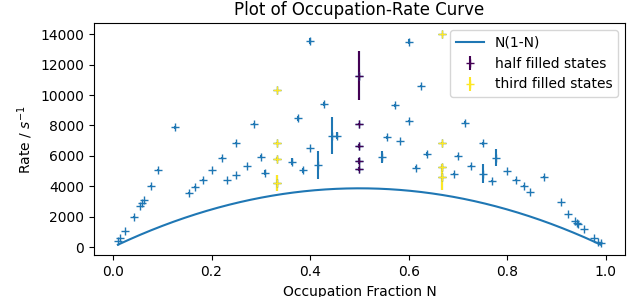
\includegraphics[width=0.7\linewidth]{Figures/Simulation/Occupation Rate Curve.png}
    \caption{Plot of the occupation-rate curve
        at 150K, with the predicted rate from half
        filled data. The rate is seen to
        tend to a constant
        value as the number of states
        \(s\rightarrow{}\infty{}\).
    }\label{fig:occupation rate curve}
\end{figure}
The rate is seen to change
at constant \(N\) as the
number of states is
increased however the asymptotic
behaviour appeared to follow the
simple form
\begin{equation}
    R(N,N) = 4 R_0 N(1-N)\label{eqn:degenerate tunnelling rate}
\end{equation}
where \(R_0\) is the
rate constant to be determined.
This is exactly the rate curve
we see in the Lindblad
analysis when hydrogen tunnelling
is paired with a single
electron transition.
Repeating the measurements at several
temperatures it was not possible
to identify any
temperature dependance of the
rate constant \(R_0\).

\subsection{Calculating \(R_0\)}\label{sec:calculating R0}
Since the rate depends only on a single
parameter \(R_0\) we are able to
extrapolate the rate from
the asymptotic
limit at a single
occupation fraction. This can
only be achieved for
\(N=\frac{1}{2}\), where
by far the largest number of
datapoints were collected (\cref{fig:half filled rate}).
\begin{figure}[htbp]
    \centering
    \begin{subfigure}{0.45\linewidth}
        \centering
        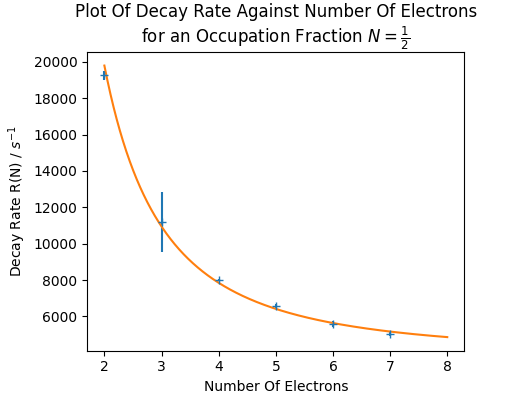
\includegraphics[width =0.9 \linewidth]{Figures/Simulation/Decay rate against electrons N=0.5.png}
        \caption{Half Filled Rates
        }\label{sub@fig:plot of half filled rates}
    \end{subfigure}
    \hfill
    \begin{subfigure}{0.45\linewidth}
        \centering
        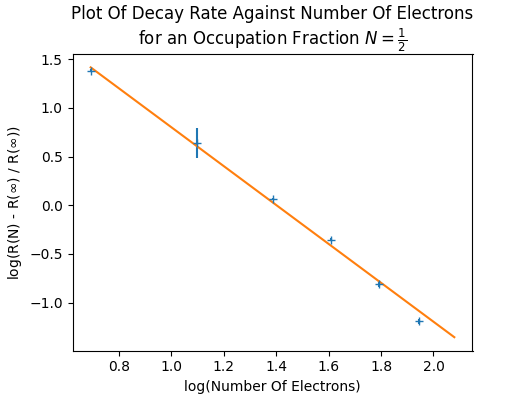
\includegraphics[width = 0.9\linewidth]{Figures/Simulation/Decay rate against electrons N=0.5 log.png}
        \caption{\(\log{}\) Half Filled Rates
        }\label{sub@fig:log plot of half fileld rates}
    \end{subfigure}
    \caption{Plot of the decay rates against
    number of electrons \(n\) for
    \(N=0.5\). The decay rates were
    fitted to
    \(R(n) = R(\infty) + {(\frac{A}{n})}^2\)
    where \(R(\infty) = R_0\) was
    found to be \(3900\pm 100s^{-1}\).
    }\label{fig:half filled rate}
\end{figure}
We are also able to extrapolate
\(R_0\) from the asymptotic
rates for states with n electrons.
As \(N\rightarrow{}0\)
we find
\(R(N,N) \sim{} 4 R_0 N = 4R_0 (\frac{n}{s})\).
We are therefore able to
use the gradient as the
number of states \(s\rightarrow{}\infty{}\)
to find \(R_0\).
Since the rate curve
is symmetric we expect
identical behaviour for
n holes, however
since the 1 electron
data was inconsistent (\cref{sub@fig:one electron rates})
we limit the analysis to 2 electron
or 2 hole data.
\begin{figure}[htbp]
    \centering
    \begin{subfigure}{0.45\linewidth}
        \centering
        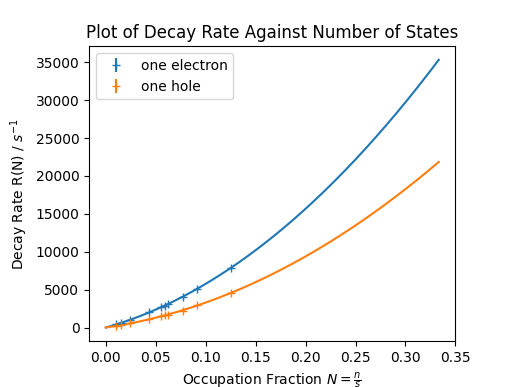
\includegraphics[width =0.9 \linewidth]{Figures/Simulation/Decay rate against occupation n=1.png}
        \caption{1 Electron Data
        }\label{sub@fig:one electron rates}
    \end{subfigure}
    \hfill
    \begin{subfigure}{0.45\linewidth}
        \centering
        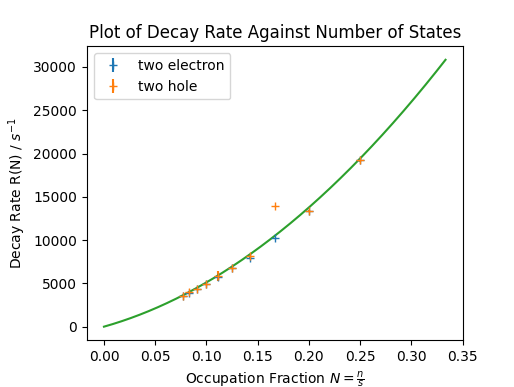
\includegraphics[width = 0.9\linewidth]{Figures/Simulation/Decay rate against occupation n=2.png}
        \caption{2 Electron Data
        }\label{sub@fig:two electron rates}
    \end{subfigure}
    \caption{Plot of the asymptotic
        form of the decay rates as \(N\rightarrow{}0\)
        at a fixed number of electrons \(n\).
        The single electron and single
        hole data is inconsistent
        (\cref{sub@fig:one electron rates}),
        however the two electron data
        was fitted to \(R(N) = 4R_0N + AN^2\)
        to give an overall rate constant
        \(R_0 = 8400\pm 600s^{-1}\). This is
        unlikely to give an accurate
        representation of the
        true decay rate, as it predicts
        a rate at \(N=0.5\)
        well above that measured even
        for \(n=5\) electrons.
    }\label{fig:small N rate}
\end{figure}
The \(N=\frac{1}{2}\) data
gave a rate constant
\(R_0 = 3900\pm 100s^{-1}\),
and for the \(n=2\) data
we find \(R_0 = 8400\pm 600s^{-1}\).
The decay rate suggested
from the \(N=2\) data is
unlikely to give an accurate
representation of the
decay rate, as it predicts
an asymptotic rate at \(N=0.5\)
well above that measured even
for \(n=5\) electrons.

\subsection{Corrected Transition Rate}\label{sec:corrected transition rate}
In the real hydrogen
system energy is conserved
during tunneling,
which leads
to the electron loosing energy
as the hydrogen transitions from
FCC to HCP sites
(\cref{sec:different hydrogen energy}).
To correct for this behaviour
we need to find the tunneling
rate from an occupation \(N\)
to an occupation \(N'\).
Due to
the arguments outlined in
\cref{app:combined tunnelling rates}
a general system with a different
forward and backward rate the
combined tunneling rate is
given by
\begin{equation}
    R(N,N') = R(N\rightarrow{}N') + R(N'\rightarrow{}N)
\end{equation}
where \(R(N\rightarrow{}N')\), \(R(N'\rightarrow{}N)\)
are the forward and backwards
tunneling rates respectively.
There are
three obvious ways to modify the tunneling
rate
\begin{align}
    R(N\rightarrow{}N') & = 2R_0N(1-N)           \label{eqn:no correction rate}     \\
    R(N\rightarrow{}N') & = 2R_0N(1-N')          \label{eqn:target correction rate}
\end{align}
all of which have the correct
limit in the case \(N=N'\),
when the forward rate is half
of the total rate given
by \cref{eqn:degenerate tunnelling rate}
\begin{equation}
    R(N\rightarrow{}N) = 2R_0N(1-N)
\end{equation}
The interpretation of these
corrections are
simple. \cref{eqn:no correction rate}
assumes the rate only depends
on the initial occupation and
\cref{eqn:target correction rate} assumes the rate
depends on the probability the
initial state is occupied
\(N\) and the final state
is unoccupied \(1-N'\). We could
also consider a correction
\begin{equation}
    R(N\rightarrow{}N') = 2R_0 \sqrt{N(1-N)N'(1-N')} \label{eqn:two hop correction}
\end{equation}
which implies a two jump process.
The electron falls to a lower band
before being promoted back into
its original location, with
each jump contributing \(\sqrt{N(1-N')}\)
to the rate. Note we have ignored functions
such as \(2R_0N'(1-N')\) which
would give the same overall rate
as \(2R_0N(1-N)\).

\subsection{Total Tunnelling Rate}
To recover the total tunneling
rate the occupation rate curve
is converted into an
energy rate using the
fermi-dirac distribution.
For \(R(N\rightarrow{}N') = 2R_0N(1-N')\)
we find
\begin{align}
    N(\epsilon)                         & = \frac{1}{1 + \exp{(\beta(\epsilon - \mu))}}                                                                         \\
    R(\epsilon \rightarrow{} \epsilon') & = 2R_0 \frac{1}{1 + \exp{(\beta(\epsilon - \mu))}}(1- \frac{1}{1 + \exp{(\beta(\epsilon' - \mu))}})                   \\
                                        & = 2R_0 \frac{\exp{(\beta(\epsilon' - \mu))}}{(1 + \exp{(\beta(\epsilon - \mu))})(1 + \exp{(\beta(\epsilon' - \mu))})}
\end{align}
where we have assumed uniform
occupation within a band.
The rate curve
(\cref{fig:tunneling rate against energy})
can then be
integrated to give an
overall tunneling rate, the results of
which are given in \cref{tab:decay rates simulated 150K}.
\begin{figure}[htbp]
    \centering
    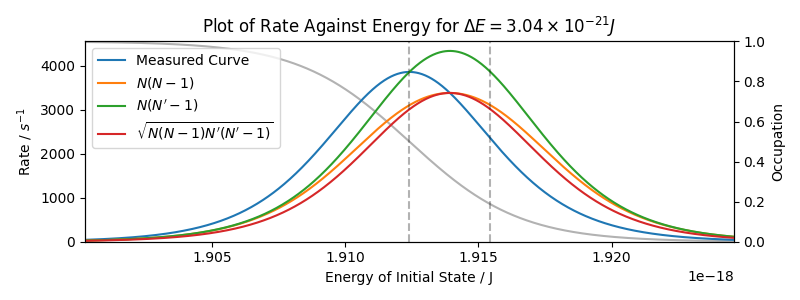
\includegraphics[width =0.9 \linewidth]{Figures/Simulation/Corrected Decay Rates.png}
    \caption{Plot of the corrected
        tunneling rate curve against
        energy. As the occupation curve
        (shown in grey) falls to 0
        the rate falls also. The corrected
        rate is seen to peak at half of the hydrogen
        energy difference above the fermi
        energy (grey dashed line).
    }\label{fig:tunneling rate against energy}
\end{figure}

\begin{table}[htbp]
    \begin{center}
        \begin{tabular}{ *{3}{c} }
            \toprule
            Rate                      & \(\frac{1}{2}\) Filled \(10^{9} s^{-1}\) & 2 Electron \(10^{9} s^{-1}\) \\
            \midrule
            Uncorrected               & \(3.6\pm 0.1\)                           & \(7.9\pm 0.6\)               \\
            \(N(1-N)\)                & \(3.6\pm 0.1\)                           & \(7.87\pm 0.6\)              \\
            \(N(1-N')\)               & \(4.3\pm 0.1\)                           & \(9.24\pm 0.7\)              \\
            \(\sqrt{N(1-N)N'(1-N')}\) & \(3.3\pm 0.1\)                           & \(7.20\pm 0.6\)              \\
            \bottomrule
        \end{tabular}
    \end{center}
    \caption{Comparison
    of decay rates at 150K.
    The tunneling rates
    taken from the
    \(\frac{1}{2}\) filled
    data is close to the
    experimental rate of
    \(3.3\times{}10^{9}s^{-1}\).
    As discussed in
    \cref{sec:calculating R0}
    the two electron decay
    represent a large
    overestimate of the
    true tunneling rate.
    }\label{tab:decay rates simulated 150K}
\end{table}

\subsection{Investigating Rate Corrections}
Given the calculated tunneling rates
it is possible to compare
the temperature dependence
with experiment.
As no temperature dependence
could be seen in the
simulation we use
the same rate constant calculated
at \(150K\) at all temperatures.
The temperature dependence
is therefore entirely
due to the corrections
made in
\cref{sec:corrected transition rate}.
The tunneling rates
plotted in
\cref{fig:simulation-experiment comparison}
show good agreement with
those measured in experiment.
\begin{figure}[htbp]
    \centering
    \begin{subfigure}{0.45\linewidth}
        \centering
        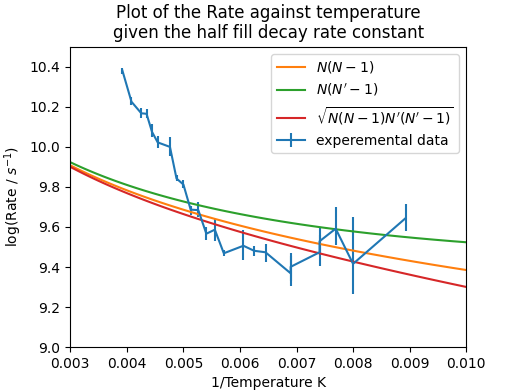
\includegraphics[width =0.9 \linewidth]{Figures/Simulation/Decay rate against temperature half fill 150K 1 spin.png}
        \caption{Half Filled Data
        }\label{sub@fig:half filled rates with experiment}
    \end{subfigure}
    \hfill
    \begin{subfigure}{0.45\linewidth}
        \centering
        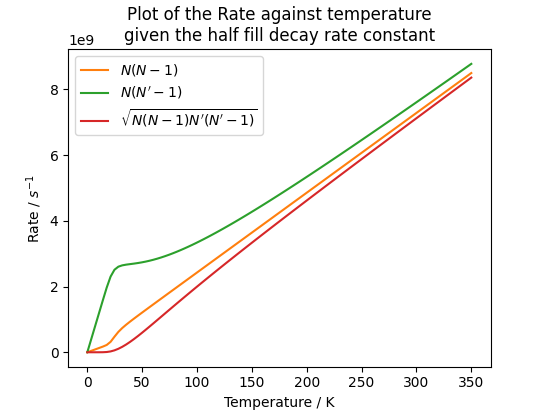
\includegraphics[width = 0.9\linewidth]{Figures/Simulation/Decay rate against temperature half fill 150K 1 spin low temp.png}
        \caption{Large Temperature Range
        }\label{sub@fig:simulation temperature dependence comparison}
    \end{subfigure}
    \caption{Plot of the decay rates
        against temperature with a comparison
        to experiment. The half
        filled data provided a good
        fit to the experimental
        tunneling rates
        (\cref{sub@fig:half filled rates with experiment}).
        The three methods of correcting
        the rate introduced in
        \cref{sec:corrected transition rate}
        gave a similar temperature
        dependence, all of which were consistent
        with experimental
        data. If we look at
        the high temperature
        limit
        \cref{sub@fig:simulation temperature dependence comparison}
        the tunneling
        rate is seen to converge
        as \(N\rightarrow{}N'\).
        The rates are seen to diverge
        at \(25K\) however this is well
        below the range of temperatures
        measured in experiment.
    }\label{fig:simulation-experiment comparison}
\end{figure}

Outside the experimentally
relevant range we see that the
tunneling rates remain
similar at all temperatures
(\cref{sub@fig:simulation temperature dependence comparison}).
Although we have no way
to predict the behaviour at
such low temperatures, the
choice \(\sqrt{N(1-N)N'(1-N')}\)
exhibits much smoother
behaviour as \(T\rightarrow{}0\).
With comparison to the lindblad
equation however
(\cref{sec:lindblad corrected tunneling})
the \(N(1-N')\)
correction seems to be the
most physically justifiable.



\subsection{Tunneling Without Self Interaction}\label{sec:tunnelling no diagonal}
In \cref{sec:different hydrogen energy}
it was found that the diagonal interaction
prevented mixing of the FCC and HCP
sites once hydrogen energy was introduced
to the experiment. It is therefore
useful to investigate the extent
to which this interaction
effects the interaction (\cref{fig:non diagonal decay rates}).
\begin{figure}[htbp]
    \centering
    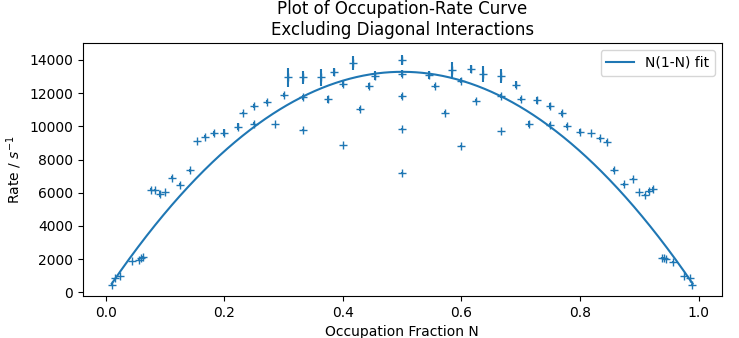
\includegraphics[width=0.7\linewidth]{Figures/Simulation/Occupation Rate Curve No Diagonal.png}
    \caption{Plot of decay rates measured without
        the inclusion of diagonal interaction.
        We see a much larger rate constant (\(R_0 \sim{} 13000 s^{-1}\)),
        and the rates are seen to
        increase (rather than
        decrease) as \(n\rightarrow{}\infty{}\).
    }\label{fig:non diagonal decay rates}
\end{figure}
The data gave
a rate constant
of \(R_0 \sim{} 13000 s^{-1}\),
more than \(3\times{}\) that seen in
the full interaction.
It is therefore
clear that this self interaction
has an important role
in the simulated
tunneling rate, and
removing such an interaction
is not a valid approach to
calculate a non-degenerate
tunneling rate.

\subsection{Simulation With Multiple Spins}



\subsection{Simulation With Multiple Hydrogen Sites}
In the real Nickel lattice the FCC and
HCP sites are arranged in a regular
lattice, such that there are \ldots
neighbouring HCP site of each FCC
hydrogen. In future investigations
it should be therefore be
possible to include the
effect of a larger number of
hydrogen sites,




\subsection{Bosons with Constrained Occupation}
To investigate the effect of fermion spin
statistics \ldots to calculate the rate
for bosons.


\section{Lindblad Assumptions}\label{sec:lindblad assumptions}

Given the results of
direct simulation it is
possible to examine
the approximations
used to arrive at
the Lindblad equation.

\subsection{Single State Tunnelling Rate}\label{sec:lindblad corrected tunneling}
When simulating the
degenerate hydrogen tunneling in
\cref{sec:degenerate tunnelling simulaton}
we found that the tunneling rate
grew proportional to \(4R_0N(1-N)\).
This corresponds exactly to the
form of the integrand of
\cref{eqn:gamma integral form},
which was proportional to
\(N_1(1 - N_3)\) where
\(E_{k3} = E_{k1} + \omega{}\),
and \(\omega{}\) is equal to
the difference in hydrogen energies
\begin{equation}
    \Gamma_{i,j, k,l}(\omega)  =\begin{aligned}[t]
        4 \int &
        \frac{d^3\vec{k}_1}{{(2\pi)}^3}
        \frac{d^3\vec{k}_3}{{(2\pi)}^3}
        V_{i,j} V_{k,l}
        N_1 (1 - N_3)
        \frac{m\delta({k_3 \pm \sqrt{k_1^2 + 2m\omega}})}{\sqrt{k_1^2 - 2m\omega}}
    \end{aligned}
\end{equation}
This suggests
that the process
is dominated
by single electron
transitions, an assumption
that was made in \cref{eqn:second order eqn of motion}
when expanding the equation
of motion to second order.

If we were to look at the
tunneling for \(\omega \neq 0\)
we find that the correct
way to modify the tunneling
rate in the simulation should
be to set
\(R(N\rightarrow{}N') = 2R_0N(1-N')\)
corresponding to \cref{eqn:target correction rate}
in
\cref{sec:corrected transition rate}.


\subsection{Final State Correction}
In \cref{sec:simulation results} we argued
that the electron state immediately
after a transition
should not effect the
dynamics of the system,
however in the Lindblad
analysis it should be possible to
properly take into account
the change in electron
distributions through
the introducing a coupling between
the electron and hydrogen density
matrices.
Although this a difficult
problem in general
if we were
to introduce a coupling
\begin{equation}
    \hat{\rho}_t = \sum_{m,n} \hat{\rho}_{m,n} \otimes {(\hat{\rho}_E)}_{m,n} \
\end{equation}
we can follow the same procedure as in
\cref{sec:the redfield assumption}
to arrive at a modified redfield equation
\begin{equation}
    \bra{m}\dot{\hat{\rho}}(t)\ket{n} = \begin{aligned}[t]
        \sum_{i,j,k, l} &
        \exp{(-i(\omega_{i,j}-\omega_{k,l})t)}
        \Gamma^{m,n}_{i,j;k, l}(\omega_{k,l})
        [S_{k, l}{\hat{\rho}(t)}_{m,n},
        S^\dagger_{i,j}]  \\
        +               &
        \exp{(i(\omega_{i,j}-\omega_{k,l}))}
        {\Gamma^*}^{m,n}_{k, l; i,j}(\omega_{i,j})
        [S_{k, l},
                {\hat{\rho}(t)}_{m,n} S^\dagger_{i,j}]
    \end{aligned}
\end{equation}
where
\begin{equation}
    \Gamma^{m,n}_{i,j, k,l}(\omega) =
    \int_0^\infty{}{
    ds \exp{(i\omega{}s)}
    Tr_{E}[E^\dagger_{i,j}(t)E_{k,l}(t-s)
    {(\hat{\rho}_E)}_{m,n}]
    }
\end{equation}
The problem is then how best to express
both the statistical and quantum uncertainty
in the form of a density matrix.

\subsection{Rotating Wave Approximation}\label{sec:rotating wave approximation}
The final approximation made in
\cref{sec:lindblad equation}
is the rotating wave approximation.
If we relax this approximation
we arrive at the expression
for the full Redfield equation given in
\cref{sec:redfield equation full solution}.
\begin{align}
    \bra{m}\dot{\hat{\rho{}}}(t) \ket{n} & = \begin{aligned}[t]
        \sum_{i,j} &
        \exp{(-i\Delta{}E_{n,j;m,i} t)}
        \Gamma_{n,j;m, i}(\omega_{m,i})
        \rho_{i,j}   \\
                   &
        -\exp{(-i\Delta{}E_{i,m;i,j} t)}
        \Gamma_{i,m;i, j}(\omega_{i,j})
        \rho_{j, n}  \\
                   &
        +\exp{(i\Delta{}E_{n,j;m,i} t)}
        \Gamma_{n,j; m, i}(\omega_{n,j})
        \rho_{i, j}  \\
                   &
        -\exp{(i\Delta{}E_{i,j;i,n} t)}
        \Gamma_{i,j; i, n}(\omega_{i,j})
        \rho_{m, j}
    \end{aligned}
\end{align}
This equation produces extra oscillations
on top of the Lindblad result, with
a characteristic timescales of
\(\frac{2\pi}{\omega_{1,0}} = 2.13\times{}10^{-13}s\). Plotting
the full solution (\cref{fig:redfield full solution})
however we see exactly the same behaviour as that
predicted by the lindblad result.
\begin{figure}[htbp]
    \centering
    \begin{subfigure}{0.45\linewidth}
        \centering
        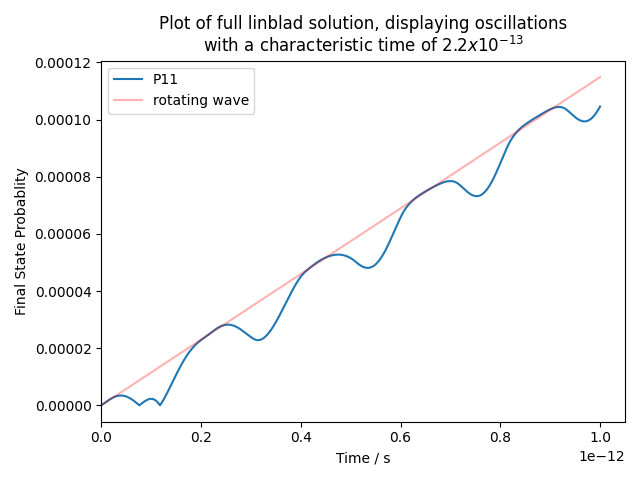
\includegraphics[width =0.9 \linewidth]{Figures/Redfield/Plot of redfield solution short time.png}
        \caption{Complete solution for small times
        }\label{fig:redfield full solution short timescales}
    \end{subfigure}
    \hfill
    \begin{subfigure}{0.45\linewidth}
        \centering
        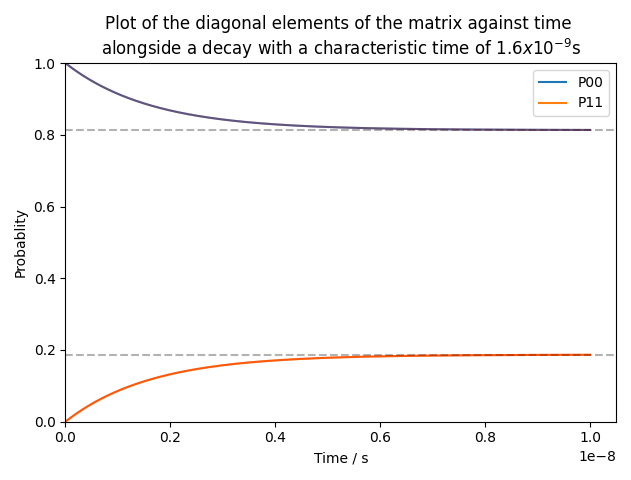
\includegraphics[width = 0.9\linewidth]{Figures/Redfield/Plot of redfield solution long time.png}
        \caption{Complete solution for long times
        }\label{fig:redfield full solution long timescales}
    \end{subfigure}
    \begin{subfigure}{0.45\linewidth}
        \centering
        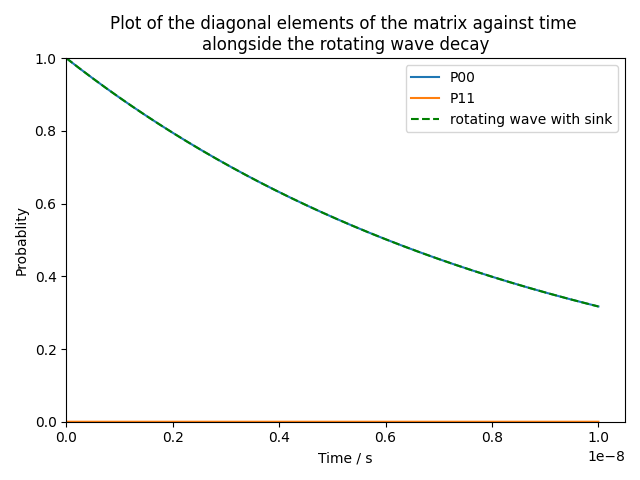
\includegraphics[width = 0.9\linewidth]{Figures/Redfield/Plot of redfield solution long time sink.png}
        \caption{Complete solution with sink
        }\label{fig:redfield full solution with sink}
    \end{subfigure}
    \caption{Plot of the full solution of the Redfield
    equation. On short timescales
    (\cref{fig:redfield full solution short timescales})
    the solution is seen to
    oscillate with a characteristic
    frequency of \(2.1\times{}10^{-13}\)s however
    at long timescales
    (\cref{fig:redfield full solution long timescales})
    the solution decays at the same rate as the
    Lindblad equation. The solution is
    also well behaved with the inclusion of
    a sink at the HCP site
    (\cref{fig:redfield full solution with sink}).
    }\label{fig:redfield full solution}
\end{figure}
In theory we should also be able
to solve the redfield equation
for multiple hydrogen sites, however
the additional computational complexity
rules this out. It is possible to
approximate the behaviour
seen in the many site model
by placing a sink at
the HCP site
(\cref{fig:redfield full solution with sink}).
In this case
we again see good
agreement with the
lindblad equation.


\subsection{Separable Density matrix}
In the analysis of the lindblad
equation we also assumed that is was possible
to factorise the density
matrix
\begin{equation}
    \hat{\rho}_t(t) = \hat{\rho}(t) \otimes \hat{\rho}_E(t)
\end{equation}
It is clear from the
initial and final
state energy distribution that
in the limit of a large
number of states the
diagonal elements are completely
uncorrelated with the
hydrogen occupation.
In the real simulation
the electron density
matrix is not diagonal,
however if we average
over a small period of time
the average is seen to
fall to zero
(\cref{fig:density matrix analysis}).
\begin{figure}[htbp]
    \centering
    \begin{subfigure}{0.45\linewidth}
        \centering
        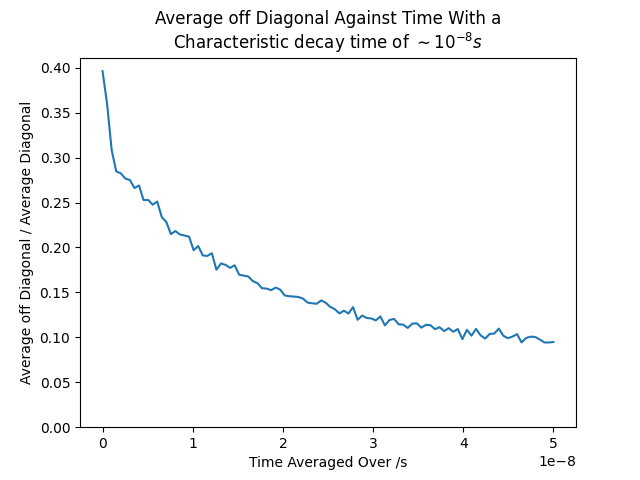
\includegraphics[width =0.9 \linewidth]{Figures/Discussion/Off Diagonal Average Matrix Element Decay.png}
        \caption{Average Off-Diagonal Decay
        }\label{sub@fig:off diagonal matrix decay}
    \end{subfigure}
    \hfill
    \begin{subfigure}{0.45\linewidth}
        \centering
        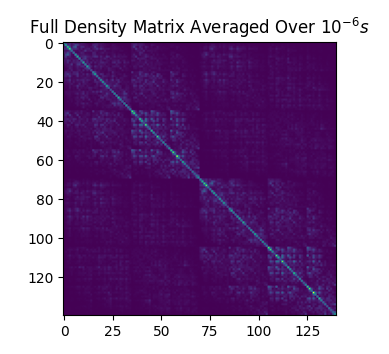
\includegraphics[width = 0.9\linewidth]{Figures/Discussion/Full average matrix 10-6s.png} %ChkTeX 8
        \caption{Averaged Density Matrix
        }\label{sub@fig:averaged density matrix}
    \end{subfigure}
    \caption{
    Plot of the average
    electron density matrix
    for a system of 5 electrons
    and 10 states
    corresponding to a tunneling time
    of \(\sim 2\times{}10^{-4}s\).
    The average off diagonal
    elements can be seen to
    fall in around
    \(\sim 2\times{}10^{-8}s\).
    }\label{fig:density matrix analysis}
\end{figure}
The approximation
therefore holds for the
same reason we are able
to ignore the off-diagonal
terms in the hydrogen density
matrix
(\cref{sec:rotating wave approximation}).
Since
the off diagonal terms
oscillate at much shorter
timescales they have
no effect on the dynamics
of the system.

\subsection{Q Dependance}
When developing a model of
the electron-hydrogen system
we assumed the interaction
hamiltonian was independent
of \(\vec{q}\).
If we instead include the full form
of the interaction potential
into \cref{eqn:gamma integral form}
we find a
lindblad rate constant that
is \(0.418 \times{}\) that
previously calculated.

We also expect a
contribution from the
\(\vec{q}\) dependance of the hydrogen overlap
fourier transform, however
to
include this we would need to
convert the discrete
DFT calculations into a continuous
function of \(\vec{q}\).
It is also possible that
the rapid oscillations
seen in the fourier transform
are simply artifacts of the
discrete DFT analysis.

For the  simulation
it will always
be necessary to assume a
\(\vec{q}\)-independent
matrix element in general,
as it is not possible
to include enough
states to properly
sample all possible initial
and final
states in 3D.
The corrections made in
the Lindblad analysis could
however be applied to the simulation,
producing an effective matrix
element depending only
on the energy difference between
two states.


\subsection{Realistic Treatment of Electrons}
In the development
of the electron-hydrogen
model we also assumed
an ideal electron gas,
with a fermi energy
of \(1.91\times{}10^{-18}J\).
The real fermi energy
of Nickel actually slightly lower,
at only \(1.24\times{} 10^{-18}J\),
possibly since the two
valence electrons are not
fully delocalised.
The fermi surface of Nickel
is also not entirely
spherical~\cite{FermiSufaceNickel},
indeed it is different
for each spin.
This is the cause of
ferromagnetic properties
within the metal~\cite{PhysRev.49.537}.

This behaviour could
be included in the
Lindblad analysis through
a modification of \cref{eqn:gamma integral form},
however it is not possible
to incorporate any
non-spherical behaviour
into the simulation
without the introduction of
an effective constant.
The complex nature of
the Nickel band-structure
means that this
could favour low or
high \(\vec{q}\) scattering,
which would lead to either an increase
or decrease in the
overall rate.
The hope
is that the surface
is sufficiently
`smoothed out' by
excitations at high
temperature such that
this is only a small
correction.

\section{Improvements and Discussion}\label{sec:improvements}










\pagebreak

\section{Conclusion}\label{sec:conclusion}
A simple model of
an electron-hydrogen
system on Ni
was developed
to explain the
incoherent tunneling
of hydrogen on a
Ni(111) surface. %ChkTeX 36

Through an application
of the Lindblad equation
a simple, closed form
expression for
the hydrogen density matrix
evolution was found,
which was used to
find an expression
for the rate at which
the combined
FCC occupation reached
equilibrium
\begin{equation}
    R   =
    12\cosh{(\frac{\beta \omega_{k,l}}{2})}
    \mathcal{C}_{1,0}\mathcal{C}_{0,1}
    \sqrt{\pi} \frac{32 k_f^2 \epsilon_0^2 \hbar^3}{\beta e^4 m_e^2}
\end{equation}
where \(\omega_{i,j}=E_i - E_j\),
\(E_i\) is the energy at site \(i\),
\(\mathcal{C}_{i,j}\) is the hydrogen
overlap fraction.
Rates extracted from
the combined FCC
occupation (\(1.8\times{}10^{-9}s^{-1}\))
next HCP occupation
(\(2.3\times{}10^{-9}s^{-1}\))
next FCC occupation
(\(1.5\times{}10^9s^{-1}\))
and initial FCC occupation
(\(2.5\times{}10^9s^{-1}\))
were all close to the
experimental rate
of \(3.3 \times{}10^{9}s^{-1}\)
at 150K\cite{Jianding-Zhu}.
The mean squared distance
was also shown to increase
linearly with time, as expected
from a decoherent stochastic
process. From this
a tunneling rate of
\(2 \times{}10^{9}s^{-1}\)
was extracted,
which was also constant with
the data at 150K.

The behaviour of the
full electron-hydrogen
model was then
investigated through
direct integration of
the Schrödinger equation.
It was found that a
simulation
including the energy of
hydrogen was not possible,
and instead a model
of degenerate hydrogen
was used to measure the
tunneling rates.
This model predicted
a tunneling rate of
\(3.6\pm 0.1\times{}10^{9}s^{-1}\)
at \(150K\)
which gave a good
prediction of the
experimental value
of
\(3.3 \times{}10^{9}s^{-1}\)\cite{Jianding-Zhu}.
A corrected tunneling rate
made with comparison
to the Lindblad equation
was
however slightly
higher at
\(4.3\pm 0.1\times{}10^{9}s^{-1}\).
The corrected rate was shown to have
a temperature dependance
consistent with that seen in
experiment
within the incoherent regime.



Results of the simulation
were applied
to assess some of the
approximations
made in the Lindblad equation.
The simulation
provided evidence
that the second order approximation
used in the Lindblad analysis
was correct,
as both methods found a
rate proportional to \(N(1-N')\).
It was also argued that
the off-diagonal
elements of the electron
density matrix
had no effect on the tunneling
rate.

To test
this model further
it should also be possible
to apply the same
techniques
to predict the
groundstate to
groundstate tunneling
of deuterium, however
there is currently
discussion
surrounding the
accuracy of the
experimental data.
The results could
also be used to
investigate the
H-Ru(111) and D-Ru(111) %ChkTeX 36
however the fermi
surface of Ruthenium
is much less spherical
and hence
the free electron
approximation may
no longer hold.

To provide more precise
predictions of the
tunneling rate
it will be necessary
to investigate the
extent to which q-dependance
of both the interaction
and the hydrogen overlap
effects the model. It is thought
that this could cause a
significant reduction in
the calculated tunneling
rate. It may also be necessary
to investigate other
sources of decoherence
within the material.

\pagebreak
\printbibliography{}
\pagebreak
\begin{appendix}
    \section{Calculating The Potential}\label{app:interaction potential calculation}
    We start from the expression for the
hydrogen potential in position basis.
TODO-Derive??
\begin{equation}
    V(\vec{r}) = \frac{e^2}{4 \pi \epsilon_0}(
    -\frac{1}{r}
    + \pi a_0^3\int{\frac{e^{-\frac{2r}{a_0}}}{
            \abs{\vec{r} - \vec{r'}}} d\vec{r}'})
\end{equation}
using two standard results
\begin{eqnarray}
    \int{\frac{1}{r} e^{i\vec{q}.\vec{r}} d^3\vec{r}}
    &=& \frac{4 \pi}{q^2}\\
    \int{e^{-\alpha r} e^{i\vec{q}.\vec{r}} d^3\vec{r}}
    &=& \frac{8 \pi \alpha}{{(\alpha^2 + q^2)}^2}\\
\end{eqnarray}
with \(\alpha = \frac{2}{a_0}\) we end up
with
\begin{eqnarray}
    V(\vec{q}) &=& \frac{e^2}{4 \pi \epsilon_0}(
    - \frac{4\pi}{q^2}
    + \frac{\pi a_0^3}{q^2}
    \frac{8 \pi \alpha}{{(\alpha^2 + q^2)}^2})\\
    &=& \frac{e^2}{\epsilon_0 q^2}(
    \frac{ \alpha^4}{{(\alpha^2 + q^2)}^2} - 1
    )
\end{eqnarray}

    \section{Combined Tunnelling Rates}\label{app:combined tunnelling rates}
    
Suppose we have a system with two states
\(x_1, x_2\)
with a forward and backwards
tunnelling rate \(\gamma_1, \gamma_2\).
We can express the equations of motion
in matrix form
\begin{align}
    \begin{pmatrix}
        \dot{x}_1 \\
        \dot{x}_2
    \end{pmatrix} = \begin{pmatrix}
        -\gamma_1 & \gamma_2   \\
        \gamma_1  & - \gamma_2
    \end{pmatrix}\begin{pmatrix}
        x_1 \\
        x_2
    \end{pmatrix}
\end{align}
from here we find the eigenvalues
and eigenvectors of the matrix.
\begin{alignat}{3}
    \lambda_1  = & -\gamma_1 - \gamma_2
                 & \Rightarrow V_1  = a\begin{pmatrix}
        1 \\
        -1
    \end{pmatrix} \\
    \lambda_2  = & 0
                 & \Rightarrow V_1  =a\begin{pmatrix}
        \frac{\gamma_2}{\gamma_1} \\
        1
    \end{pmatrix}
\end{alignat}

Given a state initially in 1
we can decompose it into these
eigenstates to find the behaviour
at a later time

\begin{alignat}{2}
    \begin{pmatrix}
        x_1(0) \\
        x_2(0)
    \end{pmatrix}              & =\begin{pmatrix}
        1 \\
        0
    \end{pmatrix} \\
                                           & =
    \frac{1}{1 + \frac{\gamma_2}{\gamma_1}}(\begin{pmatrix}
        \frac{\gamma_2}{\gamma_1} \\
        1
    \end{pmatrix} +
    \begin{pmatrix}
        1 \\
        -1
    \end{pmatrix})                                          \\
    \Rightarrow \begin{pmatrix}
        x_1(t) \\
        x_2(t)
    \end{pmatrix} & =
    \frac{1}{1 + \frac{\gamma_2}{\gamma_1}}(\begin{pmatrix}
        \frac{\gamma_2}{\gamma_1} \\
        1
    \end{pmatrix} +
    \begin{pmatrix}
        1 \\
        -1
    \end{pmatrix}\exp{(-(\gamma_1 + \gamma_2)t)})
\end{alignat}
The system therefore decays at a rate
proportional to \(\gamma_1 + \gamma_2\)
and reaches an equilibrium at
\begin{equation}
    \begin{pmatrix}
        x_1(\infty) \\
        x_2(\infty)
    \end{pmatrix}  =\frac{1}{\gamma_1 + \gamma_2} \begin{pmatrix}
        \gamma_2 \\
        \gamma_1
    \end{pmatrix}
\end{equation}


    \section{From Redfield to the Lindblad Equation}\label{app:redfield to lindblad}
    Starting from the
expression for \(\dot{\rho}(t)\)
in \cref{sec:the redfield assumption}
\begin{align}
    \dot{\hat{\rho}}(t) = \begin{aligned}[t]
        \sum_{i,j,k, l} &
        \exp{(-i(\omega_{i,j}-\omega_{k,l})t)}
        \Gamma_{i,j;k, l}(\omega_{k,l})
        [S_{k, l}\hat{\rho}(t),
        S^\dagger_{i,j}]                                       \\
        +               & \exp{(i(\omega_{i,j}-\omega_{k,l}))}
        \Gamma^*_{k, l; i,j}(\omega_{i,j})
        [S_{k, l},
            \hat{\rho}(t) S^\dagger_{i,j}]
    \end{aligned}
\end{align}
where \(S_{i,j}= \hat{a}^\dagger_i \hat{a}_j\),
\(\omega_{i,j} = E_i - E_j\), the energy of
the hydrogen atoms excluding the interaction, and
\(\Gamma\) is the Lindblad rate constant
defined in \cref{eqn:gamma definition}. To
make the following calculation easier we deal
with a single component of \(\rho \)
\begin{align}
    \bra{m}\dot{\hat{\rho}}(t) \ket{n} = \begin{aligned}[t]
        \sum_{i,j,k, l} &
        \exp{(-i\Delta{}Et)}
        \Gamma_{i,j;k, l}(\omega_{k,l})
        \bra{m}[S_{k, l}\hat{\rho}(t),
        S^\dagger_{i,j}] \ket{n}               \\
        +               & \exp{(i\Delta{}E t)}
        \Gamma^*_{k, l; i,j}(\omega_{i,j})
        \bra{m}[S_{k, l},
            \hat{\rho}(t) S^\dagger_{i,j}]\ket{n}
    \end{aligned}
\end{align}
where \(\Delta{}E = \omega_{i,j}-\omega_{k,l}\).
Focusing on the commutators we have
\begin{align}
    \bra{m}[S_{k, l}\hat{\rho}(t),
    S^\dagger_{i, j}] \ket{n} & =
    \sum_{\alpha, \beta} \rho_{\alpha, \beta}\bra{m}
    [\hat{a}^\dagger_k \hat{a}_l
        \hat{a}^\dagger_\alpha \hat{a}_\beta,
        \hat{a}^\dagger_j \hat{a}_i]
    \ket{n}                       \\
                              & =
    \sum_{\alpha, \beta} \rho_{\alpha, \beta}\bra{m}
    \hat{a}^\dagger_k \hat{a}_l
    \hat{a}^\dagger_\alpha \hat{a}_\beta
    \hat{a}^\dagger_j \hat{a}_i
    -
    \hat{a}^\dagger_j \hat{a}_i
    \hat{a}^\dagger_k \hat{a}_l
    \hat{a}^\dagger_\alpha \hat{a}_\beta
    \ket{n}                       \\
                              & =
    \sum_{\alpha, \beta} \rho_{\alpha, \beta} [
        \delta_{m, k}\delta_{l, \alpha}
        \delta_{\beta, j}\delta_{i, n}
        -\delta_{m, j}\delta_{i, k}
        \delta_{l, \alpha}\delta_{\beta, n}]
\end{align}
similarly for the second commutator
\begin{align}
    \bra{m}[S_{k, l},
    \hat{\rho}(t)S^\dagger_{i, j}] \ket{n} & =
    \sum_{\alpha, \beta} \rho_{\alpha, \beta}\bra{m}
    [\hat{a}^\dagger_k \hat{a}_l
        ,\hat{a}^\dagger_\alpha \hat{a}_\beta
        \hat{a}^\dagger_j \hat{a}_i]
    \ket{n}                                    \\
                                           & =
    \sum_{\alpha, \beta} \rho_{\alpha, \beta} [
        \delta_{m, k}\delta_{l, \alpha}
        \delta_{\beta, j}\delta_{i, n}
        -\delta_{m, \alpha}\delta_{\beta, j}
        \delta_{i, k}\delta_{l, n}]
\end{align}
subbing into the full expression for
\(\Gamma \) we find
\begin{align}
    \bra{m}\dot{\hat{\rho}}(t) \ket{n} = \begin{aligned}[t]
        \sum_{i,j,k, l, \alpha, \beta} &
        \exp{(-i\Delta{}Et)}
        \Gamma_{i,j;k, l}(\omega_{k,l})
        \rho_{\alpha, \beta} [         &
            \delta_{m, k}\delta_{l, \alpha}
        \delta_{\beta, j}\delta_{i, n}                          \\
                                       &                      &
            -\delta_{m, j}\delta_{i, k}
        \delta_{l, \alpha}\delta_{\beta, n}]                    \\
        +                              & \exp{(i\Delta{}E t)}
        \Gamma^*_{k, l; i,j}(\omega_{i,j})
        \rho_{\alpha, \beta} [         &
            \delta_{m, k}\delta_{l, \alpha}
        \delta_{\beta, j}\delta_{i, n}                          \\
                                       &                      &
            - \delta_{m, \alpha}\delta_{\beta, j}
            \delta_{i, k}\delta_{l, n}]
    \end{aligned}
\end{align}

\subsection{Rotating Wave Approximation}
To apply the rotating wave approximation we consider
two cases
\begin{itemize}
    \item \(i=j\), \(k=l\)
    \item \(i=k\), \(j=l\)
\end{itemize}
however we need to make sure we don't
double count. This is done using
the following delta
function
\(\delta_{i,j}\delta_{k,l}
+ \delta_{i,k}\delta_{j,l}
- \delta_{i,j}\delta_{k,l}
\delta_{i,k}\)
applied to each group of
\(\delta \) functions separately
\begin{align}
    (1) & =  (\delta_{i,j}\delta_{k,l}
    + \delta_{i,k}\delta_{j,l}
    - \delta_{i,j}\delta_{k,l}\delta_{i,k}) (
    \delta_{m, k}\delta_{l, \alpha}
    \delta_{\beta, j}\delta_{i, n})                          \\
        & =  (\delta_{m, k, l, \alpha}\delta_{\beta, j,i, n}
    + \delta_{i, n, m, k}\delta_{l, \alpha, \beta, j}
    - \delta_{m, k, l, \alpha, \beta, j,i, n})               \\
    (2) & =  (\delta_{i,j}\delta_{k,l}
    + \delta_{i,k}\delta_{j,l}
    - \delta_{i,j}\delta_{k,l}
    \delta_{i,k}) (
    \delta_{m, j}\delta_{i, k}
    \delta_{l, \alpha}\delta_{\beta, n})                     \\
        & =  (\delta_{m, j,i, k,l, \alpha}\delta_{\beta, n}
    + \delta_{m, j,l, \alpha}\delta_{i, k}\delta_{\beta, n}
    - \delta_{m, j,i, k, l, \alpha}\delta_{\beta, n} )       \\
    (3) & =  (\delta_{i,j}\delta_{k,l}
    + \delta_{i,k}\delta_{j,l}
    - \delta_{i,j}\delta_{k,l}
    \delta_{i,k}) (
    \delta_{m, \alpha}\delta_{\beta, j}
    \delta_{i, k}\delta_{l, n})                              \\
        & =  (\delta_{m, \alpha}\delta_{\beta, j,i, k, l, n}
    + \delta_{m, \alpha}\delta_{\beta, j,l, n}
    \delta_{i, k}
    - \delta_{m, \alpha}\delta_{\beta, j,i, k,l, n})
\end{align}
applying this to the full expression we find
\begin{align}
    \bra{m}\dot{\hat{\rho}}(t) \ket{n} & = \begin{aligned}[t]
        \sum_{i,j,k, l, \alpha, \beta} &
        \Gamma_{i,j;k, l}(\omega_{k,l})
        \rho_{\alpha, \beta} [                             \\
                                       &
            (\delta_{m, k, l, \alpha}\delta_{\beta, j,i, n}
            + \delta_{i, n, m, k}\delta_{l, \alpha, \beta, j}
        - \delta_{m, k, l, \alpha, \beta, j,i, n})         \\
                                       &
            - (    \delta_{m, j,i, k,l, \alpha}\delta_{\beta, n}
            + \delta_{m, j,l, \alpha}\delta_{i, k}\delta_{\beta, n}
        - \delta_{m, j,i, k, l, \alpha}\delta_{\beta, n})] \\
        +                              &
        \Gamma^*_{k, l; i,j}(\omega_{i,j})
        \rho_{\alpha, \beta} [                             \\
                                       &
            (\delta_{m, k, l, \alpha}\delta_{\beta, j,i, n}
            + \delta_{i, n, m, k}\delta_{l, \alpha, \beta, j}
        - \delta_{m, k, l, \alpha, \beta, j,i, n})         \\
                                       &
            - (\delta_{m, \alpha}\delta_{\beta, j,i, k, l, n}
            + \delta_{m, \alpha}\delta_{\beta, j,l, n}
            \delta_{i, k}
            - \delta_{m, \alpha}\delta_{\beta, j,i, k,l, n})]
    \end{aligned}  \\
                                       & = \begin{aligned}[t]
        \sum_{i} &
        [ (\Gamma_{n,n;m, m}(\omega_{m,m})\rho_{m, n}\delta_{i,n}
        + \Gamma_{n,i;n, i}(\omega_{n,i})\rho_{i, i}\delta_{m,n}     \\ &
        - \Gamma_{n,n;n,n}(\omega_{n,n})\rho_{n,n}\delta_{m,n,i})    \\
                 &
                - (\Gamma_{m,m;m,m}(\omega_{m,m})\rho_{m, n}\delta_{i,n}
        +\Gamma_{i,m;i, m}(\omega_{i,m})\rho_{m, n}                  \\ &
        -\Gamma_{m,m;m,m}(\omega_{m,m})\rho_{m, n}\delta_{i,n})]     \\
        +        &
        [(\Gamma^*_{m,m; n,n}(\omega_{n,n})\rho_{m, n}\delta_{i,n}
        + \Gamma^*_{m,i; m,i}(\omega_{m,i})\rho_{i, i}\delta_{n, m}  \\ &
        - \Gamma^*_{n,n,n,n}(\omega_{n,n})\rho_{n,n}\delta_{n, m,i}) \\
                 &
                - (\Gamma^*_{n,n;n,n}(\omega_{n,n})\rho_{m, n}\delta_{i,n}
        + \Gamma^*_{i, n; i,n}(\omega_{i,n})\rho_{m, n}              \\ &
                - \Gamma^*_{n,n,n,n}(\omega_{n,n})\rho_{m, n}\delta_{i, n})]
    \end{aligned}  \\
                                       & = \begin{aligned}[t]
        \sum_{i} &
        [ \Gamma_{n,n;m, m}(\omega_{m,m})\rho_{m, n}\delta_{i,n}
        + \Gamma_{n,i;n, i}(\omega_{n,i})\rho_{i, i}\delta_{m,n}    \\
                 &
                - \Gamma_{n,n;n,n}(\omega_{n,n})\rho_{n,n}\delta_{m,n,i}
        - \Gamma_{i,m;i, m}(\omega_{i,m})\rho_{m, n}]               \\
        +        &
        [ \Gamma^*_{m,m; n,n}(\omega_{n,n})\rho_{m, n}\delta_{i,n}
        + \Gamma^*_{m,i; m,i}(\omega_{m,i})\rho_{i, i}\delta_{n, m} \\
                 &
                - \Gamma^*_{n,n,n,n}(\omega_{n,n})\rho_{n,n}\delta_{n, m,i}
                - \Gamma^*_{i,n; i,n}(\omega_{i,n})\rho_{m, n}]
    \end{aligned}
\end{align}
to convert \(\Gamma^*\)
into \(\Gamma \) we use
\(\Gamma^*_{a,b,c,d} = \Gamma_{c, d, a, b}\)
\begin{align}
    \bra{m}\dot{\hat{\rho}}(t) \ket{n} & = \begin{aligned}[t]
        \sum_{i} &
        [ \Gamma_{n,n;m, m}(\omega_{m,m})\rho_{m, n}\delta_{i,n}
        + \Gamma_{n,i;n, i}(\omega_{n,i})\rho_{i, i}\delta_{m,n} \\
                 &
                - \Gamma_{n,n;n,n}(\omega_{n,n})\rho_{n,n}\delta_{m,n,i}
        - \Gamma_{i,m;i, m}(\omega_{i,m})\rho_{m, n}]            \\
        +        &
        [ \Gamma_{n,n; m, m}(\omega_{m,m})\rho_{m, n}\delta_{i,n}
        + \Gamma_{m,i;m,i}(\omega_{m,i})\rho_{i, i}\delta_{n, m} \\
                 &
                - \Gamma_{n,n,n,n}(\omega_{n,n})\rho_{n,n}\delta_{n, m,i}
                - \Gamma_{ i,n; i,n}(\omega_{n,i})\rho_{m, n}]
    \end{aligned} \\
                                       & = \begin{aligned}[t]
        \sum_{i} &
        [2 \Gamma_{n,n;m, m}(\omega_{m,m})\rho_{m, n}\delta_{i,n}
        + 2\Gamma_{n,i;n, i}(\omega_{n,i})\rho_{i, i}\delta_{m,n} \\
                 &
                - 2\Gamma_{n,n;n,n}(\omega_{n,n})\rho_{n,n}\delta_{m,n,i}
        - \Gamma_{i,m;i, m}(\omega_{i,m})\rho_{m, n}              \\
                 &
                - \Gamma_{ i,n; i,n}(\omega_{n,i})\rho_{m, n}]
    \end{aligned}
\end{align}
the second and third terms cancel
for \(i=m\), and the first and
last two terms cancel for \(m=n\)
provided \(i = n\)
\begin{align}
    \bra{m}\dot{\hat{\rho}}(t) \ket{n} & = \begin{aligned}[t]
        \sum_{i} &
        [2 \Gamma_{n,n;m, m}(\omega_{m,m})\rho_{m, n}\delta_{i,n}
        + 2\Gamma_{n,\neq n;n, \neq n}(\omega_{n,\neq n})\rho_{\neq n, \neq n}\delta_{m,n, i} \\
                 &
                - \Gamma_{i,m;i, m}(\omega_{i,m})\rho_{m, n}
                - \Gamma_{ i,n;i,n}(\omega_{n,i})\rho_{m, n}]
    \end{aligned}
\end{align}
If we take \(m=n\)
\begin{align}
    \bra{m}\dot{\hat{\rho}}(t) \ket{m} & = \begin{aligned}[t]
        \sum_{i, n\neq m} &
        [2 \Gamma_{m,m;m, m}(\omega_{m,m})\rho_{m, m}\delta_{i,m} \\ &
        + 2\Gamma_{m,n;m, n}(\omega_{m,n})\rho_{n, n}\delta_{m,i} \\
                          &
                - 2 \Gamma_{i,m;i, m}(\omega_{i,m})\rho_{m, m}]
    \end{aligned} \\
                                       & = \begin{aligned}[t]
        2\sum_{i,  n\neq m} &
        [\Gamma_{m,n;m, n}(\omega_{m,n})\rho_{n, n}\delta_{m,i} \\
                            &
                - \Gamma_{n,m;n, m}(\omega_{n,m})\rho_{m, m}\delta_{m,i}]
    \end{aligned} \\
                                       & =
    2\sum_{n\neq m}[
        \Gamma_{m,n;m, n}(\omega_{m,n})\rho_{n, n}
        - \Gamma_{n,m;n, m}(\omega_{n,m})\rho_{m, m}]
    \label{eqn:cross terms density matrix evolution}
\end{align}
If we take \(m \neq n\)
\begin{align}
    \bra{m}\dot{\hat{\rho}}(t) \ket{\neq m} & = \begin{aligned}[t]
        \sum_{i} &
        [2 \Gamma_{\neq m,\neq m;m, m}(\omega_{m,m})\rho_{m, \neq m}\delta_{i,m} \\
                 &
                - \Gamma_{i,m;i, m}(\omega_{i,m})\rho_{m, \neq m}
                - \Gamma_{ i,\neq m; i, \neq m}(\omega_{i, \neq m,})\rho_{m, \neq m}]
    \end{aligned}
\end{align}
We only have self interaction
in the diagonal elements.
If they start 0 they will
always remain zero at
later times. If we
sum over \(m\) for the
case \(n=m\) we find
the total derivative is
zero, the normalisation of
the density matrix is preserved.


\subsection{Full Solution}\label{sec:redfield equation full solution}
The full solution to the equation is
much more complicated. Starting from the
previous expression for \(\rho \) we
swap \(\Gamma^*\) for \(\Gamma \) and expand
\begin{align}
    \bra{m}\dot{\hat{\rho}}(t) \ket{n} & = \begin{aligned}[t]
        \sum_{i,j,k, l, \alpha, \beta} &
        \exp{(-i\Delta{}E_{i,j;k,l}t)}
        \Gamma_{i,j;k, l}(\omega_{k,l})
        \rho_{\alpha, \beta} [               \\ &
            \delta_{m, k}\delta_{l, \alpha}
            \delta_{\beta, j}\delta_{i, n}
            -\delta_{m, j}\delta_{i, k}
        \delta_{l, \alpha}\delta_{\beta, n}] \\
        +                              &
        \exp{(i\Delta{}E_{i,j;k,l} t)}
        \Gamma_{i,j; k, l}(\omega_{i,j})
        \rho_{\alpha, \beta} [               \\ &
            \delta_{m, k}\delta_{l, \alpha}
            \delta_{\beta, j}\delta_{i, n}
            - \delta_{m, \alpha}\delta_{\beta, j}
            \delta_{i, k}\delta_{l, n}]
    \end{aligned}                                   \\
                                       & = \begin{aligned}[t]
        \sum_{i,j} &
        \exp{(-i\Delta{}E_{n,j;m,i} t)}
        \Gamma_{n,j;m, i}(\omega_{m,i})
        \rho_{i,j}   \\
                   &
        -\exp{(-i\Delta{}E_{i,m;i,j} t)}
        \Gamma_{i,m;i, j}(\omega_{i,j})
        \rho_{j, n}  \\
                   &
        +\exp{(i\Delta{}E_{n,j;m,i} t)}
        \Gamma_{n,j; m, i}(\omega_{n,j})
        \rho_{i, j}  \\
                   &
        -\exp{(i\Delta{}E_{i,j;i,n} t)}
        \Gamma_{i,j; i, n}(\omega_{i,j})
        \rho_{m, j}
    \end{aligned}\label{eqn:full redfield solution}
\end{align}
consider the case \(m=n\)
\begin{align}
    \bra{m}\dot{\hat{\rho}}(t) \ket{m} & = \begin{aligned}[t]
        \sum_{i,j} &
        \exp{(-i\omega_{i,j} t)}
        \Gamma_{m,j;m, i}(\omega_{m,i})
        \rho_{i,j}   \\
                   &
        -\exp{(-i\omega_{j,m} t)}
        \Gamma_{i,m;i, j}(\omega_{i,j})
        \rho_{j, m}  \\
                   &
        +\exp{(i\omega_{i,j} t)}
        \Gamma_{m,j; m, i}(\omega_{m,j})
        \rho_{i, j}  \\
                   &
        -\exp{(i\omega_{m,j} t)}
        \Gamma_{i,j; i, m}(\omega_{i,j})
        \rho_{m, j}
    \end{aligned} \\
                                       & = \begin{aligned}[t]
        \sum_{i,j} &
        (\exp{(-i\omega_{i,j} t)}
        \Gamma_{m,j;m, i}(\omega_{m,i})
        +\exp{(i\omega_{i,j} t)}
        \Gamma_{m,j; m, i}(\omega_{m,j})
        )\rho_{i,j}                 \\
                   &
        -\exp{(-i\omega_{j,m} t)}
        \Gamma_{i,m;i, j}(\omega_{i,j})
        (\rho_{j, m} + \rho_{m, j}) \\
    \end{aligned}
\end{align}
we need to make sure that this
has no contribution for
\(\Gamma(0)\), as this is divergent
(see \cref{eqn:divergent expression for first integral}).
We only need
to worry about terms not already
covered by the rotating wave approximation.
This covers only one case for each part of
the expression
\begin{itemize}
    \item \(i \neq j\), \(i \neq m\) in the
          first expression
    \item \(j\neq m\), \(i \neq j\) on the
          second ect \ldots
\end{itemize}
the contribution from these
terms is then
\begin{align}
    \begin{aligned}
         & \exp{(-i\omega_{\neq m,m} t)}
        \Gamma_{m,m;m, \neq m}(\omega_{m,\neq m})
        \rho_{\neq m,m}                  \\
         &
        +\exp{(i\omega_{m,\neq m} t)}
        \Gamma_{m,\neq m; m, m}(\omega_{m,\neq m})
        \rho_{m,\neq m}                  \\
         &
        -\exp{(-i\omega_{\neq m,m} t)}
        \Gamma_{m,m;m, \neq m}(\omega_{m,\neq m})
        (\rho_{\neq m, m} + \rho_{m, \neq m})
    \end{aligned}
\end{align}
It is clear that these terms all cancel,
and the divergence of \(\Gamma \) at \(\omega = 0\)
has no effect on the diagonal terms of the
density matrix. By a similar process the same can
be shown for cross diagonal terms.

    \section{Calculating the Lindblad Rate Constant}\label{app:calculating gamma}
    Starting from the definition of gamma
(\cref{eqn:gamma definition}) and
the environment interaction hamiltonian
(\cref{eqn:split interaction hamiltonian})
we find
\begin{equation}
  \Gamma_{i,j, k,l}(\omega) =
  \int_0^\infty{}{
  ds \exp{(i\omega{}s)}
  Tr_{E}[E^\dagger_{i,j}(t)E_{k,l}(t-s)\rho_E(0)]
  }
\end{equation}
where
\begin{align}
  E_{i, j}(t) & =
  \exp{(iH_e t)}
  \sum_{k,k'} V_{i,j} \hat{b}^\dagger_{k',s'}\hat{b}_{k,s}
  \exp{(-iH_e t)}                           \\
              & = \sum_{k,k'} \hat{V}_{i,j}
  \hat{b}^\dagger_{k',s'}\hat{b}_{k,s} \exp{(i(E_k' - E_k)t)}
\end{align}
For a purely
statistical ensemble of electrons
the density matrix is
diagonal~\cite{sakurai_napolitano_2020}
\begin{equation}
  \rho_E(0) = \sum_{\{N(k)\}}
  P(\{N(k)\})
  \ket{N(k)} \bra{N(k)}
\end{equation}
where \(P(N(k)) =
\frac{1}{z}\sum_{k,s}
\exp{(-{N(k)}_s(\beta E_k - \mu))}\).

We start by expanding out the trace
over the environment
\begin{align}
  Tr_E[\dots] & = \sum_{\{N(k)\}}
  \bra{N(k)} E^\dagger_{i,j}(t)E_{k,l}(t-s) \rho_E(0) \ket{N(k)}
  \\
              & = \begin{aligned}[t]
    \sum_{\{N(k)\}, \{N'(k)\}} &
    P(\{N'(k)\}) \bra{N'(k)}  \ket{N(k)}                                               \\
                               & \bra{N(k)} E^\dagger_{i,j}(t)E_{k,l}(t-s) \ket{N'(k)}
  \end{aligned} \\
              & = \sum_{\{N(k)\}}
  P(\{N(k)\}) \bra{N(k)}
  E^\dagger_{i,j}(t)E_{k,l}(t-s) \ket{N(k)} \\
              & = \begin{aligned}[t]
    \sum_{\substack{\{N(k)\}                             \\
    k_1,s^1,k_2,s^2                                      \\
        k_3,s^3,k_4,s^4 }}
     & P(\{N(k)\}) V_{i,j} V_{k,l}                       \\
     & \exp{(i(E_1 - E_2) t)} \exp{(i(E_3 - E_4) (t-s))} \\
     & \bra{N(k)}
    \hat{b}_{k_1,s^1}^\dagger{} \hat{b}_{k_2,s^2}
    \hat{b}_{k_3,s^3}^\dagger{} \hat{b}_{k_4,s^4}
    \ket{N(k)}
  \end{aligned}
\end{align}
Where here we have used
the fact that the
potential is real, and
swapped the order of \(k_1, k_2\)
from the usual definition.
This expression is non zero
in only two cases
\begin{itemize}
  \item \(k_1=k_2, s^1=s^2\),
        \(k_3=k_4, s^3=s^4\)
  \item \(k_1=k_4, s^1=s^4\),
        \(k_3=k_2, s^3=s^2\) but
        \(k_1\neq{}k_2, s^1\neq{}s^2\)
\end{itemize}
we use the result
\begin{align}
  \bra{N(k)}
  \hat{b}_{k_1,s^1}^\dagger{}
  \hat{b}_{k_1,s^1}
  \hat{b}_{k_3,s^3}^\dagger{}
  \hat{b}_{k_3,s^3}\ket{N(k)} & = N_1 N_3       \\
  \bra{N(k)}
  \hat{b}_{k_1,s^1}^\dagger{}
  \hat{b}_{k_3,s^3}
  \hat{b}_{k_3,s^3}^\dagger{}
  \hat{b}_{k_1,s^1}\ket{N(k)} & = \bra{N(k)}
  \hat{b}_{k_1,s^1}^\dagger{}
  \hat{b}_{k_1,s^1}
  \hat{b}_{k_3,s^3}
  \hat{b}_{k_3,s^3}^\dagger{}
  \ket{N(k)}                                    \\
                              & = N_1 (1 - N_3)
\end{align}
to simplify the above sum
\begin{equation}
  Tr_E[\dots] = \begin{aligned}[t]
    \sum_{k_1,s^1,k_3,s^3 }
     & V_{i,j} V_{k,l} [ \\
     & N_1 N_3
        + N_1 (1 - N_3) \exp{(-i(E_3 - E_1)s)}]
  \end{aligned}
\end{equation}
If we then integrate over s we find
\begin{align}
  \Gamma_{i,j, k,l}(\omega) & =
  \int_0^\infty{}{
    ds \exp{(i\omega{}s)} Tr_{E}[\dots]
  }                                                      \\
  {}                        & =\begin{aligned}[t]
    \sum_{k_1,s^1,k_3,s^3,k_4,s^4 }
     & V_{i,j} V_{k,l} [ \\
     & N_1 N_3 \delta(w)
        + N_1 (1 - N_3)  \delta(w + E_1 -E_3) ]
  \end{aligned}
\end{align}
to convert these delta functions
into delta function in momentum we
use the formula
\(\delta(f(x)) =
\abs{\frac{df}{dx}}^{-1}\delta(x - x_0)\)
to give
\begin{equation}
  \delta(w + E_1 -E_3) =
  \frac{m}{\sqrt{k_1^2 - 2m\omega}}
  \delta({k_3 \pm \sqrt{k_1^2 + 2m\omega}})
\end{equation}
Note we are working in units of \(\hbar = 1\)
and the \(\delta(\omega)\) is just
constraining \(E_3 = E_4\) which is
already satisfied when \(k_3 = k_4\).
Adding this back into the expression
for \(\Gamma \) we find
\begin{align}
  \Gamma_{i,j, k,l}(\omega) & =\begin{aligned}[t]
    \sum_{k_1,s^1,k_3,s^3 }
     & V_{i,j} V_{k,l} [
    N_1 N_3 \delta_{w, 0} \frac{m}{\sqrt{k_3^2}} \\
     & + N_1 (1 - N_3)
        \frac{m}{\sqrt{k_1^2 - 2m\omega}}
        \delta({k_3 \pm \sqrt{k_1^2 + 2m\omega}}) ]
  \end{aligned}
\end{align}
To calculate these terms we
need to switch to the integral
representation. Absorbing the factors
of \(L^6\) back into the definition
of \(V_{i,j}\) we find
\begin{align}
  \Gamma_{i,j, k,l}(\omega) & =\begin{aligned}[t]
    \sum_{s^1,s^3} \int &
    \frac{d^3\vec{k}_1}{{(2\pi)}^3}
    \frac{d^3\vec{k}_3}{{(2\pi)}^3}
    V_{i,j} V_{k,l} [
    N_1 N_3 \delta_{w, 0} \frac{m}{\sqrt{k_3^2}} \\
                        & + N_1 (1 - N_3)
        \frac{m}{\sqrt{k_1^2 - 2m\omega}}
        \delta({k_3 \pm \sqrt{k_1^2 + 2m\omega}}) ]
  \end{aligned}
\end{align}
we perform the integral over k by expanding about
\(k = k_f\) noting that the value of
\(\omega \) is equal to the energy
difference of the hydrogen
\(\Gamma_{i,j, k,l}(\omega) = \Gamma_{i,j, k,l}(\omega_{k,l})\)
(see \cref{eqn:cross terms density matrix evolution}).
\begin{align}
  1 - N_3 & = \frac{1}{1 + \exp{(-\beta(E_3 - \mu))}}                                  \\
          & = \frac{1}{1 + \exp{(-\beta(E_1 + \omega - \mu))}}                         \\
          & \sim \frac{1}{2 + -\beta(E_1 + \omega - \mu)}                              \\
          & \sim \frac{1}{(1 - \frac{\beta \omega}{2})(2 + -\beta(E_1  - \mu))}        \\
          & \sim \exp{(\frac{\beta \omega}{2})}\frac{1}{1 + \exp{(-\beta(E_1 - \mu))}}
\end{align}

We then discard the first part of the integral by noting no
terms with \(\omega = 0\) appear in the
final expression for \(\dot{\rho}\), and note
\(\omega \ll k_1\) at the fermi surface.
\begin{align}
  \Gamma_{i,j, k,l}(\omega_{k,l}) & =\begin{aligned}[t]
    \sum_{s^1,s^3} \exp{(\frac{\beta \omega_{k,l}}{2})} \int &
    \frac{m{(4\pi)}^2 k_1^4 dk_1}{{(2\pi)}^6\sqrt{k_1^2 - 2m\omega}}
    V_{i,j} V_{k,l} [ N_1 (1 - N_1)]
  \end{aligned} \\
                                  & =\begin{aligned}[t]
    \sum_{s^1,s^3} \exp{(\frac{\beta \omega_{k,l}}{2})} \int &
    \frac{m k_1^3 dk_1}{4\pi^4}
    V_{i,j} V_{k,l} [ N_1 (1 - N_1)]
  \end{aligned}
\end{align}
we expand \(N_1 (1 - N_1)\) about \(k_1 = k_f\)
\begin{align}
  N_1 (1 - N_1) & = \frac{1}{1 + \exp{\beta \Delta E}}
  \frac{1}{1 + \exp{-\beta \Delta E}}                                                \\
                & \sim \frac{1}{2 + \beta \Delta E + \frac{{(\beta \Delta E)}^2}{2}}
  \frac{1}{2 - \beta \Delta E + \frac{{(\beta \Delta E)}^2}{2}}                      \\
                & = \frac{1}{4}
  \frac{1}{1 + \frac{\beta \Delta E}{2} + \frac{{(\beta \Delta E)}^2}{4}}
  \frac{1}{1 - \frac{\beta \Delta E}{2} + \frac{{(\beta \Delta E)}^2}{4}}            \\
                & \sim \begin{aligned}[t]
    \frac{1}{4}
     & (1 - \frac{\beta \Delta E}{2} - \frac{{(\beta \Delta E)}^2}{4} + {(\frac{\beta \Delta E}{2})}^2) \\
     & (1 + \frac{\beta \Delta E}{2} - \frac{{(\beta \Delta E)}^2}{4} + {(\frac{\beta \Delta E}{2})}^2)
  \end{aligned}                                    \\
                & = \frac{1}{4}(1 - \frac{{(\beta \Delta E)}^2}{4})                  \\
                & \sim \frac{1}{4}\exp{(- \frac{{(\beta \Delta E)}^2}{4})}
\end{align}
The sharp exponential decay justifies
this expansion. Going back to the
integral we have
\begin{align}
  \Gamma_{i,j, k,l}(\omega_{k,l}) & =\begin{aligned}[t]
    \sum_{s^1,s^3} \exp{(\frac{\beta \omega_{k,l}}{2})} \int &
    \frac{m k_1^3 dk_1}{{(2\pi)}^4}
    V_{i,j} V_{k,l} \exp{(- \frac{{(\beta \Delta E)}^2}{4})}
  \end{aligned} \\
                                  & =\begin{aligned}[t]
    \sum_{s^1,s^3} \exp{(\frac{\beta \omega_{k,l}}{2})} \int &
    \frac{m k_1^3 dk_1}{{(2\pi)}^4}
    V_{i,j} V_{k,l} \exp{(- \frac{{(\frac{\beta \hbar^2}{2 m}(k_1^2 - k_f^2))}^2}{4})}
  \end{aligned} \\
                                  & =\begin{aligned}[t]
    \sum_{s^1,s^3} \exp{(\frac{\beta \omega_{k,l}}{2})} \int &
    \frac{m k_f^2 du}{2{(2\pi)}^4}
    V_{i,j} V_{k,l} \exp{(- \frac{\beta^2 \hbar^4}{{(4m)}^2} u^2)}
  \end{aligned} \\
                                  & =\begin{aligned}[t]
    \sum_{s^1,s^3} \exp{(\frac{\beta \omega_{k,l}}{2})} \frac{m k_f^2 }{{(2\pi)}^4}
    V_{i,j} V_{k,l} \sqrt{\pi} \frac{2m}{\beta \hbar^2}
  \end{aligned}
\end{align}
checking the units of \(\Gamma \) we find
\begin{align}
  [\Gamma] & = {[kg]}^2[m^{-2}]{[kgm^5s^{-2}]}^2{[kgm^2s^{-2}]}^{1}{[kg m^2 s^{-1}]}^{-2} \\
           & = [{kg}^2 m^{-2} m^{6} s^{-2} {kg}^{1} m^{2} s^{-2}]                         \\
           & = [{kg}^3 m^{6}s^{-4}]
\end{align}
to recover the correct units of \(s^{-1}\) we
therefore divide by \(\hbar^3 \) which was previously
taken to be 1. We can also write
\(V_{i,j}
= \mathcal{C}_{i,j} \frac{2e^2}{\epsilon_0 \alpha^2}
= \mathcal{C}_{i,j} \frac{8 \pi^2 \epsilon_0 \hbar^4}{e^2 m^2}\)
where \(\mathcal{C}_{i,j}\) is the hydrogen
overlap factor given in \cref{sec:simplified interaction}
\begin{align}
  \Gamma_{i,j, k,l}(\omega_{k,l}) & =
  \sum_{s^1,s^3} \exp{(\frac{\beta \omega_{k,l}}{2})}
  \frac{m k_f^2 }{{(2\pi)}^4}
  \mathcal{C}_{i,j} \mathcal{C}_{k,l}
  \sqrt{\pi} \frac{2m}{\beta \hbar^5} {(\frac{8 \pi^2 \epsilon_0 \hbar^4}{e^2 m^2})}^2 \\
                                  & =
  \sum_{s^1,s^3} \exp{(\frac{\beta \omega_{k,l}}{2})}
  \mathcal{C}_{i,j} \mathcal{C}_{k,l}
  \sqrt{\pi} \frac{8 k_f^2 \epsilon_0^2 \hbar^3}{\beta e^4 m^2}
\end{align}

If we go back to calculate the
\(\omega = 0\) contribution
we find (by taking the low
temperature limit and noting
particle number is constant
with temperature)
\begin{align}
  \Gamma_{i,j, k,l}(\omega) & =
  \sum_{s^1,s^3} \int_0^{k_f}
  \frac{d^3\vec{k}_1}{{(2\pi)}^3}
  \frac{d^3\vec{k}_3}{{(2\pi)}^3}
  V_{i,j} V_{k,l} [
  N_1 N_3 \delta_{w, 0} \frac{m}{k_3}] \\
                            & =
  \sum_{s^1,s^3} \int_0^{k_f}
  \frac{4\pi k_1^2 dk_1}{{(2\pi)}^3}
  \frac{4 \pi m_e k_3 dk_3}{{(2\pi)}^3}
  V_{i,j} V_{k,l} \delta_{w, 0}        \\
                            & =
  \sum_{s^1,s^3} \frac{4\pi k_f^3 m_e}{3{(2\pi)}^3}
  \frac{2 \pi k_f^2}{{(2\pi)}^3}
  V_{i,j} V_{k,l} \delta_{w, 0}        \\
                            & =
  \sum_{s^1,s^3} \frac{4\pi k_f^3 m_e}{3{(2\pi)}^3}
  \frac{2 \pi k_f^2}{{(2\pi)}^3}
  V_{i,j} V_{k,l} \delta_{w, 0}        \\
\end{align}
If we add back in the factor of  \(\hbar^3\)
\begin{align}
  \Gamma_{i,j, k,l}(0) & =
  \sum_{s^1,s^3} \frac{4\pi k_f^3 m_e}{3\hbar^3{(2\pi)}^3}
  \frac{2 \pi k_f^2}{{(2\pi)}^3}
  \mathcal{C}_{i,j} \mathcal{C}_{k,l}
  \delta_{w, 0} {(\frac{8 \pi^2 \epsilon_0 \hbar^4}{e^2 m^2})}^2 \\
                       & =
  \sum_{s^1,s^3}
  \frac{8k_f^5 \epsilon_0^2 \hbar^5}{3e^4 m^3}
  \mathcal{C}_{i,j} \mathcal{C}_{k,l} \delta_{w, 0}
\end{align}
If we use dimensional analysis on this term
we find it is proportional to \(m^{-1}s^{-1}\).
This is because we have ignored an important
subtlety when imposing the \(\omega \) delta
function. If we had done it properly (before
setting \(k_3 = k_4\)) we would get
out an extra factor of \(L\). This term
therefore diverges as \(L \rightarrow \infty \).
\begin{align}
  \Gamma_{i,j, k,l}(0) & =
  L \sum_{s^1,s^3}
  \frac{8k_f^5 \epsilon_0^2 \hbar^5}{3e^4 m^3}
  \mathcal{C}_{i,j} \mathcal{C}_{k,l} \delta_{w, 0}
  \label{eqn:divergent expression for first integral}
\end{align}
\end{appendix}

\end{document}
